\documentclass[a4paper,12pt]{article}
\usepackage[utf8]{inputenc}
\usepackage{csquotes}
\usepackage[T1]{fontenc}
\usepackage[polish]{babel}
\usepackage{xcolor}
\usepackage{graphicx}
\usepackage{amsmath}
\usepackage{amssymb}
\usepackage{float}
\usepackage{listings}
\usepackage{hyperref}
\usepackage{enumitem}
\usepackage{longtable}
\usepackage{array}
\usepackage{booktabs}
\usepackage{tikz}
\usepackage{ragged2e}
\usepackage{geometry}
\usepackage{subcaption} 

\newcolumntype{L}[1]{>{\RaggedRight\arraybackslash}p{#1}}

\usetikzlibrary{positioning, shapes.geometric, arrows.meta}

\graphicspath{{images/}}

\lstset{
  basicstyle=\ttfamily\small,
  columns=flexible,
  keepspaces=true,
  showstringspaces=false,
  escapeinside={(*@}{@*)},
  literate={ą}{{\k{a}}}1
           {ć}{{\'{c}}}1
           {ę}{{\k{e}}}1
           {ł}{{\l{}}}1
           {ń}{{\'{n}}}1
           {ó}{{\'{o}}}1
           {ś}{{\'{s}}}1
           {ź}{{\'{z}}}1
           {ż}{{\.{z}}}1
           {Ą}{{\k{A}}}1
           {Ć}{{\'{C}}}1
           {Ę}{{\k{E}}}1
           {Ł}{{\L{}}}1
           {Ń}{{\'{N}}}1
           {Ó}{{\'{O}}}1
           {Ś}{{\'{S}}}1
           {Ź}{{\'{Z}}}1
           {Ż}{{\.{Z}}}1
           {"}{{\textquotedbl}}1
           {'}{{\textquotesingle}}1
           {`}{{\textasciigrave}}1
           {~}{{\textasciitilde}}1
           {^}{{\textasciicircum}}1
           {_}{{\textunderscore}}1
           {|}{{\textbar}}1
           {\{}{{\textbraceleft}}1
           {\}}{{\textbraceright}}1
           {[}{{[}}1
           {]}{{]}}1,
  language=SQL,
  showspaces=false,
  numbers=left,
  numberstyle=\tiny\color{gray},
  commentstyle=\color{green!60!black},
  keywordstyle=\color{blue},
  stringstyle=\color{red!80!black},
  breaklines=true,
  frame=tb,
  captionpos=b,
  tabsize=2
}

\hypersetup{
    colorlinks=true,
    linkcolor=blue,
    filecolor=magenta,
    urlcolor=cyan,
    pdftitle={Projekt hurtowni danych F1 - Kostka OLAP},
    pdfauthor={Mikołaj Kubś},
    pdfpagemode=FullScreen,
}

\title{Projekt hurtowni danych do analizy wyników i czynników wpływających na osiągnięcia kierowców Formuły 1 w latach 1950-2023}
\author{Mikołaj Kubś, 272662}
\date{\today}

\begin{document}

\maketitle
\tableofcontents
\newpage

\section{Wprowadzenie do projektu}
Proces tworzenia hurtowni danych powinien być poprzedzony zrozumieniem „potrzeb biznesu” oraz rzeczywistości (dziedziny problemowej) reprezentowanej przez dostępne zasoby danych. Realizacja poniższego zadania ma uzmysłowić występujące problemy w określonym (wybranym) wycinku rzeczywistości, a następnie umożliwić zidentyfikowanie (określenie) potrzeb, celu i możliwości analiz biznesowych, by wspierać procesy decyzyjne (podejmowanie właściwych decyzji biznesowych).

\section{Charakterystyka dziedziny problemowej, krótki opis obszaru analizy, problemy i potrzeby}

\subsection{Dziedzina problemowa}
Dziedziną problemową są Mistrzostwa Świata Formuły 1 - najbardziej prestiżowa seria wyścigów samochodowych na świecie, charakteryzująca się zaawansowaną technologią, rywalizacją na najwyższym poziomie oraz bogatą historią.

\subsection{Krótki opis obszaru analizy}
Analiza obejmuje historyczne dane dotyczące wyników kierowców i zespołów (konstruktorów) Formuły 1, począwszy od inauguracyjnego sezonu 1950 aż do końca sezonu 2023. Badane będą zarówno indywidualne osiągnięcia (pozycje, punkty, czasy), jak i dynamika zespołowa, strategie wyścigowe (np. pit-stopy), wpływ charakterystyki torów oraz, dla wybranego okresu (2018-2023), wpływ warunków atmosferycznych na przebieg i rezultaty wyścigów.

\subsection{Problemy i potrzeby}
\begin{itemize}[label=\textbullet, leftmargin=*]
  \item \textbf{Zrozumienie czynników sukcesu:} Identyfikacja kluczowych elementów (np. pozycja startowa, niezawodność bolidu, skuteczność strategii, umiejętności kierowcy, osiągi zespołu) determinujących wyniki w F1.
  \item \textbf{Analiza trendów historycznych:} Obserwacja ewolucji sportu, okresów dominacji poszczególnych zespołów i kierowców, wpływu zmian technologicznych i regulaminowych na wyniki.
  \item \textbf{Ocena strategii wyścigowych:} Analiza skuteczności różnych strategii (np. liczba i moment pit-stopów) w zależności od toru, warunków pogodowych i sytuacji na torze.
  \item \textbf{Obiektywna ocena kierowców i zespołów:} Umożliwienie porównania osiągnięć kierowców, również w kontekście siły zespołu, dla którego startowali w różnych okresach.
  \item \textbf{Potrzeby analityczne dla fanów i ekspertów:} Dostarczenie narzędzia do głębszego zrozumienia sportu, weryfikacji hipotez, tworzenia rankingów i zaawansowanych porównań wykraczających poza standardowe tabele wyników.
  \item \textbf{Analiza wpływu czynników zewnętrznych:} Zbadanie, w jakim stopniu warunki pogodowe (temperatura, opady, wiatr) korelują z wynikami wyścigów, liczbą awarii, czy pojawianiem się nieoczekiwanych rezultatów ("niespodzianek").
\end{itemize}

\section{Cel przedsięwzięcia (oczekiwania) oraz zakres analizy - badane aspekty}

\subsection{Cel przedsięwzięcia}
Głównym celem przedsięwzięcia jest zaprojektowanie i implementacja funkcjonalnej hurtowni danych wraz z kostką OLAP, która umożliwi wielowymiarową analizę wyników wyścigów Formuły 1. Narzędzie to ma pozwolić na identyfikację wzorców, trendów oraz zależności między różnymi czynnikami (charakterystyka kierowcy, zespołu, toru, strategii, pogody) a osiągnięciami sportowymi.

\subsection{Oczekiwania}
Oczekuje się, że stworzona hurtownia danych pozwoli na efektywne i intuicyjne uzyskiwanie odpowiedzi na złożone pytania analityczne. Model danych powinien być zrozumiały dla użytkownika końcowego, umożliwiając elastyczne operacje analityczne takie jak drążenie danych (drill-down, roll-up) oraz krojenie i kostkowanie (slice and dice).

\subsection{Zakres analizy - badane aspekty}
\begin{itemize}[label=\textbullet, leftmargin=*]
  \item \textbf{Wyniki indywidualne i zespołowe:} Pozycje startowe (grid) i końcowe, zdobyte punkty, czasy ukończenia wyścigów, czasy poszczególnych okrążeń (w tym najszybsze okrążenie), status ukończenia wyścigu (np. ukończony, DNF, zdyskwalifikowany).
  \item \textbf{Kierowcy:} Dane demograficzne (narodowość, data urodzenia, wiek w momencie wyścigu), historia startów, przynależność zespołowa w poszczególnych wyścigach.
  \item \textbf{Zespoły (Konstruktorzy):} Narodowość, historia startów, sumaryczne wyniki w poszczególnych wyścigach i sezonach.
  \item \textbf{Wyścigi (Events):} Sezon (rok), numer rundy w sezonie, nazwa Grand Prix, data i godzina rozpoczęcia.
  \item \textbf{Tory wyścigowe:} Charakterystyka toru (nazwa, lokalizacja, kraj, długość, typ).
  \item \textbf{Strategia wyścigowa:} Liczba odbytych pit-stopów, okrążenia, na których miały miejsce, czas trwania postojów.
  \item \textbf{Warunki pogodowe (dla lat 2018-2023):} Agregowane dane dotyczące temperatury powietrza i toru, wilgotności, ciśnienia, występowania opadów, kierunku i siły wiatru podczas wyścigu.
  \item \textbf{Wpływ regulacji (pośrednio):} Analiza zmian w wynikach, strategiach czy dominacji zespołów na przestrzeni lat może pośrednio wskazywać na wpływ zmian regulaminowych, choć same regulacje nie będą modelowane jako bezpośredni wymiar.
\end{itemize}

\section{Źródła danych (lokalizacja, format, dostępność), wstępna analiza źródeł danych}
\label{sec:zrodla_danych_final}

\begin{table}[H]
  \centering
  \caption{Źródło danych: Formula 1 World Championship (1950-2023)}
  \label{tab:zrodlo_f1_final}
  \tiny
  \begin{tabular}{|p{0.27\linewidth}|l|r|r|p{0.28\linewidth}|}
    \hline
    \textbf{Plik}                       & \textbf{Format} & \textbf{Rekordy} & \textbf{Rozmiar} & \textbf{Opis}                                                                                  \\
    \hline
    \multicolumn{5}{|l|}{\parbox{\dimexpr\linewidth-2\tabcolsep\relax}{\tiny\url{https://www.kaggle.com/datasets/rohanrao/formula-1-world-championship-1950-2020} (dane aktualizowane do 2023)}} \\
    \hline
    \texttt{circuits.csv}               & CSV             & 78               & <0.1MB           & Info o torach (ID, nazwa, kraj).                                                               \\
    \texttt{constructors.csv}           & CSV             & 212              & <0.1MB           & Info o konstr. (ID, nazwa).                                                                    \\
    \texttt{constructor\_results.csv}   & CSV             & 12625            & 0.2MB            & Wyniki konstruktorów (punkty).                                                                 \\
    \texttt{constructor\_standings.csv} & CSV             & 13391            & 0.3MB            & Pozycja konstr. po wyścigu.                                                                    \\
    \texttt{drivers.csv}                & CSV             & 861              & 0.1MB            & Info o kierowcach (ID, nazwisko).                                                              \\
    \texttt{driver\_standings.csv}      & CSV             & 34863            & 0.8MB            & Pozycja kierowców po wyścigu.                                                                  \\
    \texttt{lap\_times.csv}             & CSV             & 589k             & 16.8MB           & Czasy okrążeń.                                                                                 \\
    \texttt{pit\_stops.csv}             & CSV             & 11371            & 0.4MB            & Dane o pit-stopach.                                                                            \\
    \texttt{qualifying.csv}             & CSV             & 10494            & 0.4MB            & Wyniki kwalifikacji.                                                                           \\
    \texttt{races.csv}                  & CSV             & 1126             & 0.2MB            & Dane o wyścigach (ID, rok, tor).                                                               \\
    \texttt{results.csv}                & CSV             & 26759            & 1.6MB            & Szczegółowe wyniki kierowców.                                                                  \\
    \texttt{sprint\_results.csv}        & CSV             & 360              & <0.1MB           & Wyniki sprintów.                                                                               \\
    \texttt{status.csv}                 & CSV             & 139              & <0.1MB           & Opis statusu zakończenia.                                                                      \\
    \hline
  \end{tabular}
\end{table}

\begin{table}[H]
  \centering
  \caption{Źródło danych: Minute by Minute F1 Grand Prix Weather Data (2018-2023)}
  \label{tab:zrodlo_pogoda_final}
  \tiny
  \begin{tabular}{|p{0.27\linewidth}|l|r|r|p{0.28\linewidth}|}
    \hline
    \textbf{Plik}                      & \textbf{Format} & \textbf{Rekordy} & \textbf{Rozmiar} & \textbf{Opis}                                                                                                                                                         \\
    \hline
    \multicolumn{5}{|l|}{\parbox{\dimexpr\linewidth-2\tabcolsep\relax}{\tiny\url{https://www.kaggle.com/datasets/quantumkaze/f1-weather-dataset-2018-2023}}}                                                                                                           \\
    \hline
    \texttt{F1 Weather(2023-2018).csv} & CSV             & 18214            & 1.1MB            & Minutowe dane pogodowe dla wyścigów GP F1 (2018-2023). Kolumny: Time, AirTemp, Humidity, Pressure, Rainfall, TrackTemp, WindDirection, WindSpeed, Round Number, Year. \\
    \hline
  \end{tabular}
\end{table}

\textbf{Uwaga dotycząca danych pogodowych:} Dane z pliku \texttt{F1 Weather(2023-2018).csv} są zbierane minuta po minucie. Do celów hurtowni danych, te szczegółowe dane będą agregowane (np. poprzez uśrednianie wartości temperatury, wilgotności, prędkości wiatru; określenie dominującego kierunku wiatru; sumowanie/oznaczanie wystąpienia opadów) do poziomu całego wyścigu, aby móc je powiązać z tabelą faktów wyników wyścigów.

\subsection{Wstępna analiza źródeł}
\begin{itemize}[label=\textbullet, leftmargin=*]
  \item \textbf{Pierwsze źródło (Formula 1 World Championship):} Jest to zbiór bardzo obszerny i szczegółowy, zawierający dane historyczne od 1950 roku. Kluczowe pliki dla budowy hurtowni to:
        \begin{itemize}[label=\textendash, leftmargin=1em]
          \item \texttt{results.csv}: Główne źródło dla tabeli faktów, zawierające wyniki poszczególnych kierowców w wyścigach.
          \item \texttt{races.csv}: Dane o poszczególnych wyścigach (rok, runda, data, tor), kluczowe do łączenia z wynikami i danymi pogodowymi.
          \item \texttt{drivers.csv}, \texttt{constructors.csv}, \texttt{circuits.csv}, \texttt{status.csv}: Podstawowe źródła dla odpowiednich wymiarów (Kierowcy, Konstruktorzy, Tory, Status Zakończenia).
          \item \texttt{lap\_times.csv}, \texttt{pit\_stops.csv}: Dostarczają dodatkowych miar lub atrybutów, które mogą być włączone do tabeli faktów lub analizowane w bardziej szczegółowych kontekstach (np. średni czas pitstopu, najszybsze okrążenie).
        \end{itemize}
        Dane w tym zbiorze są generalnie dobrze zidentyfikowane przez klucze numeryczne (np. \texttt{raceId}, \texttt{driverId}, \texttt{constructorId}), co ułatwi proces łączenia tabel w procesie ETL.

  \item \textbf{Drugie źródło (Minute by Minute F1 Grand Prix Weather Data):} Ten zbiór dostarcza szczegółowych, minutowych danych pogodowych dla Grand Prix Formuły 1 w latach 2018-2023. Zawiera takie informacje jak temperatura powietrza i toru, wilgotność, ciśnienie, opady, kierunek i prędkość wiatru.
        \begin{itemize}[label=\textendash, leftmargin=1em]
          \item \textbf{Kluczowe wyzwanie i podejście:} Ze względu na wysoką granulację czasową (minuta po minucie), dane te nie mogą być bezpośrednio połączone z tabelą faktów opisującą całościowy wynik kierowcy w wyścigu. Konieczna będzie \textbf{agregacja} tych danych do poziomu całego wyścigu (lub jego kluczowych faz). W procesie ETL obliczane będą wartości średnie, minimalne, maksymalne, sumaryczne (np. dla opadów) dla każdego wyścigu.
          \item \textbf{Łączenie po agregacji:} Zagregowane dane pogodowe dla danego wyścigu zostaną połączone z głównym zbiorem danych poprzez wspólne identyfikatory: rok (\texttt{Year}) i numer rundy (\texttt{Round Number}), które są obecne w obu zbiorach (w pierwszym zbiorze w pliku \texttt{races.csv}).
        \end{itemize}
\end{itemize}

\section{Profilowanie danych (analiza jakości danych oraz ich przydatności w projekcie)}
\label{sec:profilowanie_danych_final}
Poniżej przedstawiono szczegółowe profilowanie danych dla każdego pliku CSV wykorzystywanego w projekcie. Analiza opiera się na raportach wygenerowanych przez bibliotekę `ydata-profiling`. Analizowane będą tylko przydatne atrybuty.

\subsection{Plik: \texttt{circuits.csv}}
\begin{longtable}{|p{0.03\linewidth}|p{0.18\linewidth}|p{0.15\linewidth}|p{0.2\linewidth}|p{0.3\linewidth}|}
  \caption{Profilowanie danych dla \texttt{circuits.csv}} \label{tab:profil_circuits}                                                                                                \\
  \hline
  \tiny\textbf{Lp.} & \tiny\textbf{Atrybut} & \tiny\textbf{Typ danych} & \tiny\textbf{Zakres wartości}         & \tiny\textbf{Uwagi - ocena jakości danych i przydatności}           \\
  \hline
  \endfirsthead
  \multicolumn{5}{c}%
  {{\tiny\bfseries \tablename\ \thetable{} -- ciąg dalszy}}                                                                                                                          \\
  \hline
  \tiny\textbf{Lp.} & \tiny\textbf{Atrybut} & \tiny\textbf{Typ danych} & \tiny\textbf{Zakres wartości}         & \tiny\textbf{Uwagi - ocena jakości danych i przydatności}           \\
  \hline
  \endhead
  \hline \multicolumn{5}{|r|}{{\tiny Ciąg dalszy na następnej stronie}}                                                                                                              \\
  \endfoot
  \hline
  \endlastfoot
  \tiny 1.          & \tiny `circuitId`     & \tiny Numeric (Real)     & \tiny Min: 1, Max: 80                 & \tiny Klucz główny. Unikalny, brak braków. Jakość wysoka.           \\
  \tiny 2.          & \tiny `circuitRef`    & \tiny Text               & \tiny Unikalne wartości               & \tiny Tekstowy ID. Unikalny, brak braków. Jakość wysoka. Przydatny. \\
  \tiny 3.          & \tiny `name`          & \tiny Text               & \tiny Unikalne wartości               & \tiny Nazwa toru. Unikalny, brak braków. Jakość wysoka. Przydatny.  \\
  \tiny 4.          & \tiny `location`      & \tiny Text               & \tiny 75 unikalnych (z 77)            & \tiny Miasto. Brak braków. Jakość dobra. Przydatny.                 \\
  \tiny 5.          & \tiny `country`       & \tiny Categorical        & \tiny 35 unikalnych                   & \tiny Kraj. Brak braków. Jakość dobra. Kluczowy dla wymiaru geo.    \\
  \tiny 6.          & \tiny `lat`           & \tiny Numeric (Real)     & \tiny Min: -37.85, Max: 57.27         & \tiny Szer. geogr. Unikalna, brak braków. Jakość wysoka. Przydatna. \\
  \tiny 7.          & \tiny `lng`           & \tiny Numeric (Real)     & \tiny Min: -118.19, Max: 144.97       & \tiny Dł. geogr. Unikalna, brak braków. Jakość wysoka. Przydatna.   \\
  \tiny 8.          & \tiny `alt`           & \tiny Numeric (Real)     & \tiny Min: -7, Max: 2227; 2.6\% Zeros & \tiny Wysokość n.p.m. Brak braków. Jakość dobra.                    \\
\end{longtable}

\subsection{Plik: \texttt{constructors.csv}}
\begin{longtable}{|p{0.03\linewidth}|p{0.18\linewidth}|p{0.15\linewidth}|p{0.2\linewidth}|p{0.3\linewidth}|}
  \caption{Profilowanie danych dla \texttt{constructors.csv}} \label{tab:profil_constructors}                                                                                  \\
  \hline
  \tiny\textbf{Lp.} & \tiny\textbf{Atrybut}  & \tiny\textbf{Typ danych} & \tiny\textbf{Zakres wartości} & \tiny\textbf{Uwagi - ocena jakości danych i przydatności}            \\
  \hline
  \endfirsthead
  \multicolumn{5}{c}%
  {{\tiny\bfseries \tablename\ \thetable{} -- ciąg dalszy}}                                                                                                                    \\
  \hline
  \tiny\textbf{Lp.} & \tiny\textbf{Atrybut}  & \tiny\textbf{Typ danych} & \tiny\textbf{Zakres wartości} & \tiny\textbf{Uwagi - ocena jakości danych i przydatności}            \\
  \hline
  \endhead
  \hline \multicolumn{5}{|r|}{{\tiny Ciąg dalszy na następnej stronie}}                                                                                                        \\
  \endfoot
  \hline
  \endlastfoot
  \tiny 1.          & \tiny `constructorId`  & \tiny Numeric (Real)     & \tiny Min: 1, Max: 215        & \tiny Klucz główny. Unikalny, brak braków. Jakość wysoka.            \\
  \tiny 2.          & \tiny `constructorRef` & \tiny Text               & \tiny Unikalne wartości       & \tiny Tekstowy ID. Unikalny, brak braków. Jakość wysoka.             \\
  \tiny 3.          & \tiny `name`           & \tiny Text               & \tiny Unikalne wartości       & \tiny Nazwa. Unikalny, brak braków. Jakość wysoka. Kluczowy atrybut. \\
  \tiny 4.          & \tiny `nationality`    & \tiny Categorical        & \tiny 24 unikalne             & \tiny Narodowość. Brak braków. Jakość dobra. Ważny atrybut.          \\
\end{longtable}

\subsection{Plik: \texttt{drivers.csv}}
\begin{longtable}{|p{0.03\linewidth}|p{0.18\linewidth}|p{0.15\linewidth}|p{0.2\linewidth}|p{0.3\linewidth}|}
  \caption{Profilowanie danych dla \texttt{drivers.csv}} \label{tab:profil_drivers}                                                                                   \\
  \hline
  \tiny\textbf{Lp.} & \tiny\textbf{Atrybut} & \tiny\textbf{Typ danych} & \tiny\textbf{Zakres wartości} & \tiny\textbf{Uwagi - ocena jakości danych i przydatności}    \\
  \hline
  \endfirsthead
  \multicolumn{5}{c}%
  {{\tiny\bfseries \tablename\ \thetable{} -- ciąg dalszy}}                                                                                                           \\
  \hline
  \tiny\textbf{Lp.} & \tiny\textbf{Atrybut} & \tiny\textbf{Typ danych} & \tiny\textbf{Zakres wartości} & \tiny\textbf{Uwagi - ocena jakości danych i przydatności}    \\
  \hline
  \endhead
  \hline \multicolumn{5}{|r|}{{\tiny Ciąg dalszy na następnej stronie}}                                                                                               \\
  \endfoot
  \hline
  \endlastfoot
  \tiny 1.          & \tiny `driverId`      & \tiny Numeric (Real)     & \tiny Min: 1, Max: 862        & \tiny Klucz główny. Unikalny, brak braków. Jakość wysoka.    \\
  \tiny 2.          & \tiny `driverRef`     & \tiny Text               & \tiny Unikalne wartości       & \tiny Tekstowy ID. Unikalny, brak braków. Jakość wysoka.     \\
  \tiny 3.          & \tiny `number`        & \tiny Numeric (Real)     & \tiny Min: 2, Max: 99         & \tiny Nr startowy. **93.1\% braków!** Niska/średnia jakość.  \\
  \tiny 4.          & \tiny `code`          & \tiny Text               & \tiny 97 unikalnych           & \tiny Kod kierowcy. **87.9\% braków!** Niska/średnia jakość. \\
  \tiny 5.          & \tiny `forename`      & \tiny Text               & \tiny 478 unikalnych          & \tiny Imię. Brak braków. Jakość wysoka. Kluczowy.            \\
  \tiny 6.          & \tiny `surname`       & \tiny Text               & \tiny 802 unikalne            & \tiny Nazwisko. Brak braków. Jakość wysoka. Kluczowy.        \\
  \tiny 7.          & \tiny `dob`           & \tiny DateTime           & \tiny Min: 1896, Max: 2005    & \tiny Data urodzenia. Brak braków. Jakość wysoka. Kluczowy.  \\
  \tiny 8.          & \tiny `nationality`   & \tiny Categorical        & \tiny 43 unikalne             & \tiny Narodowość. Brak braków. Jakość dobra. Ważny atrybut.  \\
\end{longtable}

\subsection{Plik: \texttt{lap\_times.csv}}
\begin{longtable}{|p{0.03\linewidth}|p{0.18\linewidth}|p{0.15\linewidth}|p{0.18\linewidth}|p{0.32\linewidth}|}
  \caption{Profilowanie danych dla \texttt{lap\_times.csv}} \label{tab:profil_lap_times}                                                                                                             \\
  \hline
  \tiny\textbf{Lp.} & \tiny\textbf{Atrybut} & \tiny\textbf{Typ danych} & \tiny\textbf{Zakres wartości} & \tiny\textbf{Uwagi - ocena jakości danych i przydatności}                                   \\
  \hline
  \endfirsthead
  \multicolumn{5}{c}%
  {{\tiny\bfseries \tablename\ \thetable{} -- ciąg dalszy}}                                                                                                                                          \\
  \hline
  \tiny\textbf{Lp.} & \tiny\textbf{Atrybut} & \tiny\textbf{Typ danych} & \tiny\textbf{Zakres wartości} & \tiny\textbf{Uwagi - ocena jakości danych i przydatności}                                   \\
  \hline
  \endhead
  \hline \multicolumn{5}{|r|}{{\tiny Ciąg dalszy na następnej stronie}}                                                                                                                              \\
  \endfoot
  \hline
  \endlastfoot
  \tiny 1.          & \tiny `raceId`        & \tiny Numeric (Real)     & \tiny Min: 1, Max: 1144       & \tiny Klucz obcy. Brak braków. Jakość wysoka.                                               \\
  \tiny 2.          & \tiny `driverId`      & \tiny Numeric (Real)     & \tiny Min: 1, Max: 862        & \tiny Klucz obcy. Brak braków. Jakość wysoka.                                               \\
  \tiny 3.          & \tiny `lap`           & \tiny Numeric (Real)     & \tiny Min: 1, Max: 87         & \tiny Nr okrążenia. Brak braków. Jakość wysoka.                                             \\
  \tiny 4.          & \tiny `position`      & \tiny Numeric (Real)     & \tiny Min: 1, Max: 24         & \tiny Pozycja na okrążeniu. Brak braków. Jakość wysoka.                                     \\
  \tiny 5.          & \tiny `time`          & \tiny Text               & \tiny np. "1:38.109"          & \tiny Czas okr. (tekst). Brak braków. Wymaga parsowania. Jakość wysoka.                     \\
  \tiny 6.          & \tiny `milliseconds`  & \tiny Numeric (Real)     & \tiny Min: 55404, Max: 7.5M   & \tiny Czas okr. (ms). Brak braków. Jakość średnia. Kluczowa miara. Max wartość to anomalia. \\
\end{longtable}

\subsection{Plik: \texttt{pit\_stops.csv}}
\begin{longtable}{|p{0.03\linewidth}|p{0.18\linewidth}|p{0.15\linewidth}|p{0.18\linewidth}|p{0.32\linewidth}|}
  \caption{Profilowanie danych dla \texttt{pit\_stops.csv}} \label{tab:profil_pit_stops}                                                                                                       \\
  \hline
  \tiny\textbf{Lp.} & \tiny\textbf{Atrybut} & \tiny\textbf{Typ danych} & \tiny\textbf{Zakres wartości} & \tiny\textbf{Uwagi - ocena jakości danych i przydatności}                             \\
  \hline
  \endfirsthead
  \multicolumn{5}{c}%
  {{\tiny\bfseries \tablename\ \thetable{} -- ciąg dalszy}}                                                                                                                                    \\
  \hline
  \tiny\textbf{Lp.} & \tiny\textbf{Atrybut} & \tiny\textbf{Typ danych} & \tiny\textbf{Zakres wartości} & \tiny\textbf{Uwagi - ocena jakości danych i przydatności}                             \\
  \hline
  \endhead
  \hline \multicolumn{5}{|r|}{{\tiny Ciąg dalszy na następnej stronie}}                                                                                                                        \\
  \endfoot
  \hline
  \endlastfoot
  \tiny 1.          & \tiny `raceId`        & \tiny Numeric (Real)     & \tiny Min: 841, Max: 1144     & \tiny Klucz obcy. Brak braków. Dane od raceId > 840. Jakość wysoka.                   \\
  \tiny 2.          & \tiny `driverId`      & \tiny Numeric (Real)     & \tiny Min: 1, Max: 862        & \tiny Klucz obcy. Brak braków. Jakość wysoka.                                         \\
  \tiny 3.          & \tiny `stop`          & \tiny Numeric (Real)     & \tiny Min: 1, Max: 70         & \tiny Nr pit stopu. Brak braków. Max 70 to anomalia. Jakość ok.                       \\
  \tiny 4.          & \tiny `lap`           & \tiny Numeric (Real)     & \tiny Min: 1, Max: 78         & \tiny Okrążenie pit stopu. Brak braków. Jakość wysoka.                                \\
  \tiny 5.          & \tiny `time`          & \tiny DateTime           & \tiny HH:MM:SS                & \tiny Godzina pit stopu z dodatkową datą. Wymaga parsowania. Dobra jakość.            \\
  \tiny 6.          & \tiny `duration`      & \tiny Text               & \tiny np. "26.898"            & \tiny Czas trwania (tekst). Brak braków. Wymaga parsowania. Jakość dobra.             \\
  \tiny 7.          & \tiny `milliseconds`  & \tiny Numeric (Real)     & \tiny Min: 12.9k, Max: 3M     & \tiny Czas trwania (ms). Brak braków. Jakość wysoka. Max wartość (51min) to anomalia. \\
\end{longtable}

\subsection{Plik: \texttt{races.csv}}
\begin{longtable}{|p{0.03\linewidth}|p{0.15\linewidth}|p{0.13\linewidth}|p{0.2\linewidth}|p{0.35\linewidth}|}
  \caption{Profilowanie danych dla \texttt{races.csv}} \label{tab:profil_races}                                                                                                                                                              \\
  \hline
  \tiny\textbf{Lp.} & \tiny\textbf{Atrybut} & \tiny\textbf{Typ danych} & \tiny\textbf{Zakres wartości} & \tiny\textbf{Uwagi - ocena jakości danych i przydatności}                                                                           \\
  \hline
  \endfirsthead
  \multicolumn{5}{c}%
  {{\tiny\bfseries \tablename\ \thetable{} -- ciąg dalszy}}                                                                                                                                                                                  \\
  \hline
  \tiny\textbf{Lp.} & \tiny\textbf{Atrybut} & \tiny\textbf{Typ danych} & \tiny\textbf{Zakres wartości} & \tiny\textbf{Uwagi - ocena jakości danych i przydatności}                                                                           \\
  \hline
  \endhead
  \hline \multicolumn{5}{|r|}{{\tiny Ciąg dalszy na następnej stronie}}                                                                                                                                                                      \\
  \endfoot
  \hline
  \endlastfoot
  \tiny 1.          & \tiny `raceId`        & \tiny Numeric (Real)     & \tiny Min: 1, Max: 1144       & \tiny Klucz główny. Unikalny, brak braków. Jakość wysoka.                                                                           \\
  \tiny 2.          & \tiny `year`          & \tiny Numeric (Real)     & \tiny Min: 1950, Max: 2024    & \tiny Rok. Brak braków. Jakość wysoka. Kluczowy.                                                                                    \\
  \tiny 3.          & \tiny `round`         & \tiny Numeric (Real)     & \tiny Min: 1, Max: 24         & \tiny Runda. Brak braków. Jakość wysoka. Kluczowy.                                                                                  \\
  \tiny 4.          & \tiny `circuitId`     & \tiny Numeric (Real)     & \tiny Min: 1, Max: 80         & \tiny Klucz obcy. Brak braków. Jakość wysoka. Kluczowy.                                                                             \\
  \tiny 5.          & \tiny `name`          & \tiny Text               & \tiny 54 unikalne             & \tiny Nazwa GP. Brak braków. Jakość wysoka.                                                                                         \\
  \tiny 6.          & \tiny `date`          & \tiny DateTime           & \tiny Min: 1950, Max: 2024    & \tiny Data wyścigu. Unikalna, brak braków. Jakość wysoka. Kluczowa.                                                                 \\
  \tiny 7.          & \tiny `time`          & \tiny DateTime           & \tiny HH:MM:SS; Braki 65.0\%  & \tiny Godzina startu. Błędnie jako DateTime. Dużo braków - dane tylko od 2005 roku. Wymaga parsowania. Może być kluczowy do pogody. \\
\end{longtable}

\subsection{Plik: \texttt{results.csv}}
\begin{longtable}{|p{0.03\linewidth}|p{0.17\linewidth}|p{0.13\linewidth}|p{0.2\linewidth}|p{0.33\linewidth}|}
  \caption{Profilowanie danych dla \texttt{results.csv}} \label{tab:profil_results}                                                                                                                                           \\
  \hline
  \tiny\textbf{Lp.} & \tiny\textbf{Atrybut}   & \tiny\textbf{Typ danych} & \tiny\textbf{Zakres wartości}            & \tiny\textbf{Uwagi - ocena jakości danych i przydatności}                                               \\
  \hline
  \endfirsthead
  \multicolumn{5}{c}%
  {{\tiny\bfseries \tablename\ \thetable{} -- ciąg dalszy}}                                                                                                                                                                   \\
  \hline
  \tiny\textbf{Lp.} & \tiny\textbf{Atrybut}   & \tiny\textbf{Typ danych} & \tiny\textbf{Zakres wartości}            & \tiny\textbf{Uwagi - ocena jakości danych i przydatności}                                               \\
  \hline
  \endhead
  \hline \multicolumn{5}{|r|}{{\tiny Ciąg dalszy na następnej stronie}}                                                                                                                                                       \\
  \endfoot
  \hline
  \endlastfoot
  \tiny 1.          & \tiny `resultId`        & \tiny Numeric (Real)     & \tiny Min: 1, Max: 26764                 & \tiny Klucz główny. Unikalny, brak braków. Jakość wysoka.                                               \\
  \tiny 2.          & \tiny `raceId`          & \tiny Numeric (Real)     & \tiny Min: 1, Max: 1144                  & \tiny Klucz obcy. Brak braków. Jakość wysoka.                                                           \\
  \tiny 3.          & \tiny `driverId`        & \tiny Numeric (Real)     & \tiny Min: 1, Max: 862                   & \tiny Klucz obcy. Brak braków. Jakość wysoka.                                                           \\
  \tiny 4.          & \tiny `constructorId`   & \tiny Numeric (Real)     & \tiny Min: 1, Max: 215                   & \tiny Klucz obcy. Brak braków. Jakość wysoka.                                                           \\
  \tiny 5.          & \tiny `number`          & \tiny Numeric (Real)     & \tiny Min: 0, Max: 208; Braki <0.1\%     & \tiny Nr startowy. Bardzo małe braki. Jakość dobra.                                                     \\
  \tiny 6.          & \tiny `grid`            & \tiny Numeric (Real)     & \tiny Min: 0, Max: 34; 6.1\% to zera     & \tiny Pozycja startowa. Brak braków. Jakość wysoka. Kluczowa miara. Dziwnie dużo 0.                     \\
  \tiny 7.          & \tiny `position`        & \tiny Numeric (Real)     & \tiny Min: 1, Max: 33; Braki 40.9\%      & \tiny Pozycja końcowa. Dużo braków (DNF). `positionOrder` lepsze.                                       \\
  \tiny 9.          & \tiny `positionOrder`   & \tiny Numeric (Real)     & \tiny Min: 1, Max: 39                    & \tiny Uporządkowana pozycja. Brak braków. Jakość wysoka. Lepsza do rankingu.                            \\
  \tiny 10.         & \tiny `points`          & \tiny Numeric (Real)     & \tiny Min: 0, Max: 50; 69.5\% to zera    & \tiny Punkty. Brak braków. Jakość wysoka. Kluczowa miara.                                               \\
  \tiny 11.         & \tiny `laps`            & \tiny Numeric (Real)     & \tiny Min: 0, Max: 200; 9.5\% Zeros      & \tiny Ukończone okrążenia. Brak braków. Jakość wysoka. Miara.                                           \\
  \tiny 12.         & \tiny `time`            & \tiny Text               & \tiny np. "1:30:00", "+5s"; Braki 71.3\% & \tiny Czas. Dużo braków. Wymaga parsowania. `milliseconds` lepsze. Niska jakość.                        \\
  \tiny 13.         & \tiny `milliseconds`    & \tiny Numeric (Real)     & \tiny Min: 526, Max: 15M; Braki 71.3\%   & \tiny Czas (ms). Dużo braków. Jakość wysoka (dla niepustych). Kluczowa miara.                           \\
  \tiny 14.         & \tiny `fastestLap`      & \tiny Numeric (Real)     & \tiny Min: 1, Max: 85; Braki 69.2\%      & \tiny Nr najszybszego okrążenia. Dużo braków. Jakość średnia.                                           \\
  \tiny 15.         & \tiny `rank`            & \tiny Numeric (Real)     & \tiny Min: 0, Max: 24; Braki 68.2\%      & \tiny Ranking najszybszego okrażenia. Dużo braków. Jakość średnia.                                      \\
  \tiny 16.         & \tiny `fastestLapTime`  & \tiny DateTime           & \tiny MM:SS.mmm; Braki 69.2\%            & \tiny Czas najszybszego okrążenia. Błędnie jako DateTime. Wymaga parsowania. Dużo braków. Niska jakość. \\
  \tiny 17.         & \tiny `fastestLapSpeed` & \tiny Numeric (Real)     & \tiny Min: 89, Max: 257; Braki 69.2\%    & \tiny Prędkość najszybszego okrążenia. Dużo braków. Jakość średnia.                                     \\
  \tiny 18.         & \tiny `statusId`        & \tiny Numeric (Real)     & \tiny Min: 1, Max: 141                   & \tiny Klucz obcy do `status.csv`. Brak braków. Jakość wysoka. Kluczowy.                                 \\
\end{longtable}

\subsection{Plik: \texttt{status.csv}}
\begin{longtable}{|p{0.03\linewidth}|p{0.18\linewidth}|p{0.15\linewidth}|p{0.2\linewidth}|p{0.3\linewidth}|}
  \caption{Profilowanie danych dla \texttt{status.csv}} \label{tab:profil_status}                                                                                            \\
  \hline
  \tiny\textbf{Lp.} & \tiny\textbf{Atrybut} & \tiny\textbf{Typ danych} & \tiny\textbf{Zakres wartości} & \tiny\textbf{Uwagi - ocena jakości danych i przydatności}           \\
  \hline
  \endfirsthead
  \multicolumn{5}{c}%
  {{\tiny\bfseries \tablename\ \thetable{} -- ciąg dalszy}}                                                                                                                  \\
  \hline
  \tiny\textbf{Lp.} & \tiny\textbf{Atrybut} & \tiny\textbf{Typ danych} & \tiny\textbf{Zakres wartości} & \tiny\textbf{Uwagi - ocena jakości danych i przydatności}           \\
  \hline
  \endhead
  \hline \multicolumn{5}{|r|}{{\tiny Ciąg dalszy na następnej stronie}}                                                                                                      \\
  \endfoot
  \hline
  \endlastfoot
  \tiny 1.          & \tiny `statusId`      & \tiny Numeric (Real)     & \tiny Min: 1, Max: 141        & \tiny Klucz główny. Unikalny, brak braków. Jakość wysoka.           \\
  \tiny 2.          & \tiny `status`        & \tiny Text               & \tiny Unikalne wartości       & \tiny Opis statusu. Unikalny, brak braków. Jakość wysoka. Kluczowy. \\
\end{longtable}

\subsection{Plik: \texttt{weather.csv}}
\begin{longtable}{|p{0.03\linewidth}|p{0.18\linewidth}|p{0.15\linewidth}|p{0.18\linewidth}|p{0.32\linewidth}|}
  \caption{Profilowanie danych dla \texttt{weather.csv}} \label{tab:profil_weather}                                                                                                                                                                                                                                           \\
  \hline
  \tiny\textbf{Lp.} & \tiny\textbf{Atrybut}                                & \tiny\textbf{Typ danych}                                                                    & \tiny\textbf{Zakres wartości} & \tiny\textbf{Uwagi - ocena jakości danych i przydatności}                                                          \\
  \hline
  \endfirsthead
  \multicolumn{5}{c}%
  {{\tiny\bfseries \tablename\ \thetable{} -- ciąg dalszy}}                                                                                                                                                                                                                                                                   \\
  \hline
  \tiny\textbf{Lp.} & \tiny\textbf{Atrybut}                                & \tiny\textbf{Typ danych}                                                                    & \tiny\textbf{Zakres wartości} & \tiny\textbf{Uwagi - ocena jakości danych i przydatności}                                                          \\
  \hline
  \endhead
  \hline \multicolumn{5}{|r|}{{\tiny Ciąg dalszy na następnej stronie}}                                                                                                                                                                                                                                                       \\
  \endfoot
  \hline
  \endlastfoot
  \tiny 1.          & \tiny `Time`                                         & \tiny Text                                                                                  & \tiny `timedelta`             & \tiny Czas odniesienia. Brak braków. Wymaga parsowania - trzeba usunąć "0 days" z przodu. Jakość wysoka. Kluczowy. \\
  \tiny 2.          & \tiny `AirTemp`                                      & \tiny Numeric (Real)                                                                        & \tiny Min: 8.9, Max: 37.2     & \tiny Temperatura powietrza. Brak braków. Jakość wysoka. Kluczowa miara.                                           \\
  \tiny 3.          & \tiny `Humidity`                                     & \tiny Numeric (Real)                                                                        & \tiny Min: 5, Max: 97.5       & \tiny Wilgotność. Brak braków. Jakość wysoka. Kluczowa miara.                                                      \\
  \tiny 4.          & \tiny `Pressure`                                     & \tiny Numeric (Real)                                                                        & \tiny Min: 778.5, Max: 1023.5 & \tiny Ciśnienie. Brak braków. Jakość wysoka. Miara.                                                                \\
  \tiny 5.          & \tiny `Rainfall`                                     & \tiny Boolean                                                                               & \tiny True/False              & \tiny Opady. Brak braków. Jakość wysoka. Kluczowa miara.                                                           \\
  \tiny 6.          & \tiny `TrackTemp`                                    & \tiny Numeric (Real)                                                                        & \tiny Min: 13.8, Max: 67      & \tiny Temp. toru. Brak braków. Jakość wysoka. Kluczowa miara.                                                      \\
  \tiny 7.          & \tiny `WindDirection`                                & \tiny Numeric (Real)                                                                        & \tiny Min: 0, Max: 359        & \tiny Kier. wiatru. Brak braków. Jakość wysoka. Miara.                                                             \\
  \tiny 8.          & \tiny `WindSpeed`                                    & \tiny Numeric (Real)                                                                        & \tiny Min: 0, Max: 10.1       & \tiny Prędkość wiatru. Brak braków. Jakość wysoka. Kluczowa miara.                                                 \\
  \tiny 9.          & \tiny `Round Number`                                 & \tiny Numeric (Real)                                                                        & \tiny Min: 1, Max: 22         & \tiny Nr rundy. Brak braków. Jakość wysoka. Kluczowy do łączenia.                                                  \\
  \tiny 10.         & \tiny `Year`                                         & \tiny Numeric (Real)                                                                        & \tiny Min: 2018, Max: 2023    & \tiny Rok. Brak braków. Jakość wysoka. Kluczowy do łączenia.                                                       \\
  \tiny             & \multicolumn{3}{l|}{\tiny \textbf{Dodatkowa uwaga:}} & \tiny Raport wskazuje 3.2\% zduplikowanych wierszy. Należy zbadać i usunąć przed agregacją.                                                                                                                                                      \\
\end{longtable}

\section{Definicja typów encji/klas, związków, diagram klas}
\label{sec:definicja_encji_final}
Projektowana hurtownia danych będzie oparta na schemacie gwiazdy, z centralną tabelą faktów \texttt{Fact\_Result} oraz otaczającymi ją tabelami wymiarów.

\subsection{Tabela faktów: \texttt{Fact\_Result}}
\begin{itemize}[label=\textbullet, leftmargin=*]
  \item \textbf{Opis:} Reprezentuje pojedynczy, całościowy wynik kierowcy w danym wyścigu Grand Prix. Ziarnistość tabeli to jeden rekord per kierowca per wyścig.
  \item \textbf{Klucze obce (referencje do wymiarów):}
        \begin{itemize}[label=\textendash, leftmargin=1em]
          \item \texttt{RaceKey} (FK do Dim\_Race)
          \item \texttt{DriverKey} (FK do Dim\_Driver)
          \item \texttt{ConstructorKey} (FK do Dim\_Constructor)
          \item \texttt{CircuitKey} (FK do Dim\_Circuit)
          \item \texttt{DateKey} (FK do Dim\_Time - data wyścigu)
          \item \texttt{WeatherKey} (FK do Dim\_Weather, może być NULL dla wyścigów sprzed 2018)
          \item \texttt{StatusKey} (FK do Dim\_Status)
        \end{itemize}
  \item \textbf{Miary (przykładowe):}
        \begin{itemize}[label=\textendash, leftmargin=1em]
          \item \texttt{PointsScored} (DECIMAL) - zdobyte punkty (addytywna)
          \item \texttt{LapsCompleted} (INT) - liczba ukończonych okrążeń (addytywna)
          \item \texttt{NumberOfPitStops} (INT, wyliczana z \texttt{pit\_stops.csv}) - liczba pit-stopów (addytywna)
          \item \texttt{PitStopsTotalTimeMS} (BIGINT, wyliczana z \texttt{pit\_stops.csv}) - łączny czas pit-stopów w milisekundach (addytywna)
          \item \texttt{RaceTimeMS} (BIGINT, nullable) - czas ukończenia wyścigu w milisekundach (póładdytywna)
          \item \texttt{GridPosition} (INT) - pozycja startowa (nieaddytywna)
          \item \texttt{FinalPositionOrder} (INT) - numeryczna pozycja na mecie (nieaddytywna)
          \item \texttt{PositionOrderChange} (INT) - różnica między pozycją startową a finalną (nieaddytywna)
          \item \texttt{FastestLapTimeMS} (BIGINT, nullable) - czas najszybszego okrążenia kierowcy w wyścigu (nieaddytywna)
          \item \texttt{RankFastestLap} (INT, nullable) - ranking najszybszego okrążenia kierowcy w wyścigu (nieaddytywna)
          \item \texttt{FastestLapTopSpeedMS} (BIGINT, nullable) - maksymalna szybkość podczas najszybszego okrążenia (nieaddytywna)
          \item \texttt{AgeAtRace} (INT) - wiek kierowcy w momencie wyścigu (nieaddytywna)
        \end{itemize}
\end{itemize}

\section{Min. 10 wielowymiarowych zestawień}
\label{sec:zestawienia}
Poniżej przedstawiono przykładowe wielowymiarowe zestawienia, które będzie można utworzyć po wdrożeniu kostki OLAP:
\begin{enumerate}[label=\arabic*., wide, labelindent=0pt]
  \item \textbf{Wpływ pozycji startowej na wynik:} Średnia pozycja na mecie i procent zwycięstw dla każdej pozycji startowej (grid), z możliwością filtrowania wg toru i sezonu.
  \item \textbf{Stabilność kierowców:} Średnie punkty na wyścig, liczba miejsc na podium i zwycięstw na sezon dla wybranych (najbardziej znanych) kierowców na przestrzeni ich kariery.
  \item \textbf{"Gwiazdy w słabych zespołach":} Identyfikacja kierowców, którzy regularnie zdobywali punkty lub wysokie pozycje dla zespołów z końca stawki (np. porównanie wyników kierowcy ze średnią zespołu).
  \item \textbf{Ewolucja strategii pit-stopów:} Średnia liczba pit-stopów i ich łącznego czasu na wyścig i ich wpływ na wynik, analizowana wg toru, sezonu i warunków pogodowych.
  \item \textbf{Dominacja zespołów:} Procent wygranych wyścigów i zdobytych punktów przez poszczególne zespoły w sezonach.
  \item \textbf{Trendy narodowościowe:} Liczba kierowców, zwycięzców i mistrzów świata z podziałem na narodowości i kontynenty, na przestrzeni dekad.
  \item \textbf{Pogoda a niezawodność:} Korelacja między zagregowanymi warunkami pogodowymi (np. wysokie/niskie temperatury, opady deszczu) a liczbą nieukończonych wyścigów (DNF) z powodu awarii lub wypadków.
  \item \textbf{Pogoda a nieoczekiwane wyniki:} Analiza, czy deszczowe lub zmienne warunki pogodowe częściej przynoszą nieoczekiwane wyniki (np. zwycięzcy spoza czołowych zespołów, kierowcy z dalszych pozycji na podium).
  \item \textbf{Pojedynki zespołowe:} Porównanie wyników (punkty, pozycje w kwalifikacjach i wyścigach) kierowców startujących w tym samym zespole w danym sezonie.
  \item \textbf{Charakterystyka torów a wyniki:} Jak zmieniały się czasy ukończenia torów z biegiem lat? Które tory generują najwięcej/najmniej zmian pozycji?
  \item \textbf{Analiza DNF:} Najczęstsze przyczyny nieukończenia wyścigu (na podstawie \texttt{Dim\_Status}) dla poszczególnych zespołów i na przestrzeni sezonów, z uwzględnieniem wpływu pogody.
  \item \textbf{Wpływ wieku kierowcy na osiągnięcia:} Korelacja między wiekiem kierowcy a jego wynikami (np. średnia liczba punktów na sezon, częstotliwość błędów, szybkość na pojedynczym okrążeniu).
\end{enumerate}

\section{Implementacja bazy danych (konceptualny model danych - DDL)}
\label{sec:implementacja_db_final}
Poniżej przedstawiono skrypt SQL tworzący strukturę tabel wymiarów i faktów zgodnie z zaproponowanym modelem. Klucze obce, więzy integralności są zdefiniowane.

\begin{lstlisting}[language=SQL, caption=Konceptualny DDL dla hurtowni danych F1, label=lst:ddl_full_f1_final]
CREATE TABLE Dim_Driver (
    DriverKey INT PRIMARY KEY,
    DriverID_NK INT UNIQUE,             
    DriverRef VARCHAR(255) UNIQUE,
    FirstName VARCHAR(255),
    LastName VARCHAR(255),
    FullName VARCHAR(510),            
    DateOfBirth DATE,
    Nationality VARCHAR(255),
    Continent VARCHAR(255)
);

CREATE TABLE Dim_Constructor (
    ConstructorKey INT PRIMARY KEY,  
    ConstructorID_NK INT UNIQUE,  
    ConstructorRef VARCHAR(255) UNIQUE,
    Name VARCHAR(255),
    Nationality VARCHAR(255),
    Continent VARCHAR(255)
);

CREATE TABLE Dim_Race (
    RaceKey INT PRIMARY KEY,        
    RaceID_NK INT UNIQUE,              
    YearSeason INT,
    RoundNumberInSeason INT,
    RaceNameOfficial VARCHAR(255)
);

CREATE TABLE Dim_Circuit (
    CircuitKey INT PRIMARY KEY,       
    CircuitID_NK INT UNIQUE,         
    CircuitRef VARCHAR(255) UNIQUE,
    CircuitName VARCHAR(255),
    LocationCity VARCHAR(255),
    CountryName VARCHAR(255),
    Latitude DECIMAL(9,6),
    Longitude DECIMAL(9,6),
    Altitude INT
);

CREATE TABLE Dim_Time (
    DateKey INT PRIMARY KEY,          
    FullDate DATE UNIQUE,
    Year INT,
    Quarter INT,
    Month INT,
    MonthName VARCHAR(50),
    DayOfMonth INT,
    DayOfWeekName VARCHAR(50),
    WeekOfYear INT
);

CREATE TABLE Dim_Weather (
    WeatherKey INT PRIMARY KEY,   
    AvgAirTempCelsius DECIMAL(5,2),
    MinAirTempCelsius DECIMAL(5,2),
    MaxAirTempCelsius DECIMAL(5,2),
    AvgTrackTempCelsius DECIMAL(5,2),
    AvgHumidityPercent DECIMAL(5,2),
    DidRainOccur BIT,               -- 0 lub 1
    TotalRainfallMM DECIMAL(6,2),
    AvgWindSpeedKmph DECIMAL(5,2),
    MaxWindSpeedKmph DECIMAL(5,2),
    DominantWindDirection VARCHAR(50),  -- Np. N, NW, S (kategoria)
);

CREATE TABLE Dim_Status (
    StatusKey INT PRIMARY KEY,         
    StatusID_NK INT UNIQUE,             
    StatusDescription VARCHAR(255),
    StatusCategory VARCHAR(100)         -- Np. Finished, Accident, Failure
);

CREATE TABLE Fact_Result (
    RaceKey INT,
    DriverKey INT,
    ConstructorKey INT,
    CircuitKey INT,                
    DateKey INT,                     
    WeatherKey INT NULL,            
    StatusKey INT,

    -- Miary
    PointsScored DECIMAL(5,1),
    LapsCompleted INT,
    NumberOfPitStops INT NULL,
    PitStopsTotalTimeMS BIGINT NULL,
    RaceTimeMS BIGINT NULL,
    GridPosition INT,
    FinalPositionOrder INT,
    PositionOrderChange INT,            -- (GridPosition - FinalPositionOrder)
    FastestLapTimeMS BIGINT NULL,
    RankFastestLap INT NULL,
    FastestLapTopSpeed DECIMAL(6,2) NULL,
	  AgeAtRace DECIMAL(5,3) NULL,

    FOREIGN KEY (RaceKey) REFERENCES Dim_Race(RaceKey),
    FOREIGN KEY (DriverKey) REFERENCES Dim_Driver(DriverKey),
    FOREIGN KEY (ConstructorKey) REFERENCES Dim_Constructor(ConstructorKey),
    FOREIGN KEY (CircuitKey) REFERENCES Dim_Circuit(CircuitKey),
    FOREIGN KEY (DateKey) REFERENCES Dim_Time(DateKey),
    FOREIGN KEY (WeatherKey) REFERENCES Dim_Weather_Aggregated(WeatherKey),
    FOREIGN KEY (StatusKey) REFERENCES Dim_Status(StatusKey)
);
\end{lstlisting}

\section{Wnioski}
Proponowany projekt hurtowni danych dla wyników Formuły 1 w latach 1950-2023 ma na celu stworzenie kompleksowego narzędzia analitycznego. Wykorzystanie dwóch głównych źródeł danych - szczegółowych wyników historycznych oraz minutowych danych pogodowych (agregowanych do poziomu wyścigu) dla ostatnich sezonów - pozwoli na przeprowadzenie wielowymiarowych analiz, które mogą odkryć interesujące wzorce, trendy i zależności.

\subsection{Główne korzyści}
\begin{itemize}[label=\textbullet, leftmargin=*]
  \item Umożliwienie odpowiedzi na szeroki zakres pytań analitycznych dotyczących strategii, osiągów kierowców i zespołów oraz wpływu czynników zewnętrznych, w tym pogody.
  \item Dostarczenie spójnego i zintegrowanego zbioru danych, ułatwiającego analizy porównawcze na przestrzeni lat i między różnymi aspektami wyścigów.
  \item Możliwość wizualizacji i eksploracji danych F1 w sposób bardziej zaawansowany niż standardowe tabele wyników, wspierając podejmowanie decyzji i głębsze zrozumienie sportu.
\end{itemize}

\subsection{Potencjalne wyzwania}
\begin{itemize}[label=\textbullet, leftmargin=*]
  \item \textbf{Agregacja i integracja danych pogodowych:} Precyzyjne zdefiniowanie logiki agregacji minutowych danych pogodowych oraz zapewnienie poprawnego określenia zakresu czasowego wyścigu dla tej agregacji.
  \item \textbf{Jakość danych źródłowych:} Obsługa brakujących wartości (NULL), niespójności formatów (np. czasów) oraz potencjalnych wartości odstających w obu zbiorach danych.
  \item \textbf{Zakres danych pogodowych:} Analizy wykorzystujące szczegółowe dane pogodowe będą ograniczone do sezonów 2018-2023. Można by za pomocą API pozyskać brakujące dane (poza temperaturą nawierzchni). Ciekawą alternatywą byłoby też użycie prostej estymacji temperatury nawierzchni z danych pogodowych - mało danych treningowych, ale wysoce prawdopodobne jest to, że temperature nawierzchni jest bardzo powiązana z np. temperaturą z ostatnich x godzin z coraz mniejszymi wagami, plus uwzględnienie wilgotności / deszczu.
  \item \textbf{Interpretacja historyczna i zmiany regulaminowe:} Uwzględnienie znaczących zmian w regulaminach F1 (np. systemy punktacji, aerodynamika, specyfikacje opon) przy interpretacji wyników i trendów z różnych epok sportu.
  \item \textbf{Obsługa stref czasowych:} Zapewnienie spójności w przetwarzaniu danych czasowych, szczególnie przy łączeniu `timedelta` z danych pogodowych z czasem startu wyścigu.
\end{itemize}

\section{Architektura i narzędzia procesu ETL}

\subsection{Struktura procesu ETL}
Proces ETL został zorganizowany w ramach jednego projektu SSIS, zawierającego dedykowane pakiety dla ładowania poszczególnych tabel wymiarów oraz tabeli faktów. Dodatkowo, zaimplementowano pakiet główny (master
package) koordynujący uruchamianie poszczególnych pakietów w odpowiedniej kolejności (najpierw wymiary, następnie fakty), aby zapewnić integralność referencyjną.

Struktura pakietów SSIS:
\begin{itemize}
  \item \_Dim\_Circuit.dtsx
  \item \_Dim\_Driver.dtsx
  \item \_Dim\_Constructor.dtsx
  \item \_Dim\_Race.dtsx
  \item \_Dim\_Status.dtsx
  \item \_Dim\_Weather.dtsx
  \item \_Fact\_Result.dtsx
  \item \_Dim\_Time.dtsx
\end{itemize}

\subsection{Mapa logiczna ETL}

% --- DIM_DRIVER ---
\subsubsection{Mapowanie atrybutów: Dim\_Driver}
\begin{footnotesize}
  \begin{longtable}{|L{3.5cm}|L{3.5cm}|L{3cm}|L{7cm}|}
    \caption{Mapowanie ETL dla tabeli Dim\_Driver} \label{tab:map_dim_driver}
    \\
    \toprule
    \textbf{Atrybut} & \textbf{Źródła}                                & \textbf{Kolumna źródła}          & \textbf{Transformacje i uwagi}
    \\
    \midrule
    \endfirsthead
    \multicolumn{4}{c}%
    {{\bfseries \tablename\ \thetable{} -- Kontynuacja z poprzedniej strony}}
    \\
    \toprule
    \textbf{Atrybut} & \textbf{Źródła}                                & \textbf{Kolumna źródła}          & \textbf{Transformacje i uwagi}
    \\
    \midrule
    \endhead
    \midrule
    \multicolumn{4}{|r|}{{Kontynuacja na następnej stronie}}
    \\
    \midrule
    \endfoot
    \bottomrule
    \endlastfoot

    DriverKey        & -                                              & -                                & SQL Server IDENTITY(1,1). Klucz zastępczy.
    \\
    \hline
    DriverID\_NK     & drivers.xlsx                                   & driverId                         & Bezpośrednio. Klucz naturalny ze źródła.                                 \\
    \hline
    FirstName        & drivers.xlsx                                   & forename                         & Bezpośrednio.                                                            \\
    \hline
    LastName         & drivers.xlsx                                   & surname                          & Bezpośrednio.                                                            \\
    \hline
    FullName         & drivers.xlsx                                   & forename, surname                & Derived Column: forename + " " + surname. Pełne imię i nazwisko          \\
    \hline
    DateOfBirth      & drivers.xlsx                                   & dob                              & Bezpośrednio.                                                            \\
    \hline
    CountryName      & drivers.xlsx, Helper\_Nationality              & nationality                      & Lookup do Helper\_NationalityCountries.                                  \\
    \hline
    Continent        & Helper\_Nationality \newline Helper\_Continent & CountryName poprzednio obliczone & Lookup do Helper\_CountryContinents z poprzednio obliczonego CountryName \\
  \end{longtable}
\end{footnotesize}

% --- DIM_CONSTRUCTOR ---
\subsubsection{Mapowanie atrybutów: Dim\_Constructor}
\begin{footnotesize}
  \begin{longtable}{|L{3.5cm}|L{3.5cm}|L{3cm}|L{7cm}|}
    \caption{Mapowanie ETL dla tabeli Dim\_Constructor} \label{tab:map_dim_constructor}                                                                                       \\
    \toprule
    \textbf{Atrybut}  & \textbf{Źródła}                                               & \textbf{Kolumna źródła}         & \textbf{Transformacje i uwagi}                      \\
    \midrule
    \endfirsthead
    \multicolumn{4}{c}%
    {{\bfseries \tablename\ \thetable{} -- Kontynuacja z poprzedniej strony}}                                                                                                 \\
    \toprule
    \textbf{Atrybut}  & \textbf{Źródła}                                               & \textbf{Kolumna źródła}         & \textbf{Transformacje i uwagi}                      \\
    \midrule
    \endhead
    \midrule
    \multicolumn{4}{|r|}{{Kontynuacja na następnej stronie}}                                                                                                                  \\
    \midrule
    \endfoot
    \bottomrule
    \endlastfoot
    ConstructorKey    & -                                                             & -                               & SQL Server IDENTITY(1,1). Klucz zastępczy.          \\
    \hline
    ConstructorID\_NK & constructors.xlsx                                             & constructorId                   & Bezpośrednio. Klucz naturalny.                      \\
    \hline
    Name              & constructors.xlsx                                             & name                            & Bezpośrednio.                                       \\
    \hline
    CountryName       & constructors.xlsx \newline Helper\_Nationality                & nationality                     & Lookup nationality do Helper\_NationalityCountries. \\
    \hline
    Continent         & {Helper\_Continent \newline poprzednio obliczone CountryName} & CountryName wcześniej obliczone & Lookup CountryName do Helper\_CountryContinent      \\
  \end{longtable}
\end{footnotesize}

% --- DIM_RACE ---
\subsubsection{Mapowanie atrybutów: Dim\_Race}
\begin{footnotesize}
  \begin{longtable}{|L{3.5cm}|L{3.5cm}|L{3cm}|L{7cm}|}
    \caption{Mapowanie ETL dla tabeli Dim\_Race} \label{tab:map_dim_race}                                        \\
    \toprule
    \textbf{Atrybut}    & \textbf{Źródła} & \textbf{Kolumna źródła} & \textbf{Transformacje i uwagi}             \\
    \midrule
    \endfirsthead
    \multicolumn{4}{c}%
    {{\bfseries \tablename\ \thetable{} -- Kontynuacja z poprzedniej strony}}                                    \\
    \toprule
    \textbf{Atrybut}    & \textbf{Źródła} & \textbf{Kolumna źródła} & \textbf{Transformacje i uwagi}             \\
    \midrule
    \endhead
    \midrule
    \multicolumn{4}{|r|}{{Kontynuacja na następnej stronie}}                                                     \\
    \midrule
    \endfoot
    \bottomrule
    \endlastfoot
    RaceKey             & -               & -                       & SQL Server IDENTITY(1,1). Klucz zastępczy. \\
    \hline
    RaceID\_NK          & races.xlsx      & raceId                  & Bezpośrednio. Klucz naturalny.             \\
    \hline
    CircuitID\_NK       & races.xlsx      & circuitId               & Bezpośrednio. NK obwodu dla tego wyścigu.  \\
    \hline
    YearSeason          & races.xlsx      & year                    & Bezpośrednio.                              \\
    \hline
    RoundNumberInSeason & races.xlsx      & round                   & Bezpośrednio.                              \\
    \hline
    RaceNameOfficial    & races.xlsx      & name                    & Bezpośrednio.                              \\
    \hline
    Date                & races.xlsx      & date                    & Bezpośrednio. Używana do DateKey w Fact.   \\
  \end{longtable}
\end{footnotesize}

% --- DIM_CIRCUIT ---
\subsubsection{Mapowanie atrybutów: Dim\_Circuit}
\begin{footnotesize}
  \begin{longtable}{|L{3.5cm}|L{3.5cm}|L{3cm}|L{7cm}|}
    \caption{Mapowanie ETL dla tabeli Dim\_Circuit} \label{tab:map_dim_circuit}                               \\
    \toprule
    \textbf{Atrybut} & \textbf{Źródła} & \textbf{Kolumna źródła} & \textbf{Transformacje i uwagi}             \\
    \midrule
    \endfirsthead
    \multicolumn{4}{c}%
    {{\bfseries \tablename\ \thetable{} -- Kontynuacja z poprzedniej strony}}                                 \\
    \toprule
    \textbf{Atrybut} & \textbf{Źródła} & \textbf{Kolumna źródła} & \textbf{Transformacje i uwagi}             \\
    \midrule
    \endhead
    \midrule
    \multicolumn{4}{|r|}{{Kontynuacja na następnej stronie}}                                                  \\
    \midrule
    \endfoot
    \bottomrule
    \endlastfoot
    CircuitKey       & -               & -                       & SQL Server IDENTITY(1,1). Klucz zastępczy. \\
    \hline
    CircuitID\_NK    & circuits.xlsx   & circuitId               & Bezpośrednio. Klucz naturalny.             \\
    \hline
    CircuitName      & circuits.xlsx   & name                    & Bezpośrednio.                              \\
    \hline
    LocationCity     & circuits.xlsx   & location                & Bezpośrednio.                              \\
    \hline
    CountryName      & circuits.xlsx   & country                 & Bezpośrednio.                              \\
  \end{longtable}
\end{footnotesize}

% --- DIM_TIME ---
\subsubsection{Mapowanie atrybutów: Dim\_Time}
\begin{footnotesize}
  \begin{longtable}{|L{3.5cm}|L{3.5cm}|L{3cm}|L{7cm}|}
    \caption{Mapowanie ETL dla tabeli Dim\_Time} \label{tab:map_dim_time}
    \\
    \toprule
    \textbf{Atrybut} & \textbf{Źródła}                     & \textbf{Kolumna}             & \textbf{Transformacje i uwagi}
    \\
    \midrule
    \endfirsthead
    \multicolumn{4}{c}%
    {{\bfseries \tablename\ \thetable{} -- Kontynuacja z poprzedniej strony}}
    \\
    \toprule
    \textbf{Atrybut} & \textbf{Źródła}                     & \textbf{Kolumna}             & \textbf{Transformacje i uwagi}
    \\
    \midrule
    \endhead
    \midrule
    \multicolumn{4}{|r|}{{Kontynuacja na następnej stronie}}
    \\
    \midrule
    \endfoot
    \bottomrule
    \endlastfoot
    DateKey          & Fact\_Result                        & Distinct DateKey             & Distinct z DateKey w Fact\_Result. PK, YYYYMMDD INT.                                   \\
    \hline
    FullDate         & Dim\_Time                           & DateKey wcześniej obliczone  & Derived column: rok, miesiąc i dzień za pomocą modulo i dzielenia z DateKey.           \\
    \hline
    Year             & Dim\_Time                           & FullDate wcześniej obliczone & Derived Column: DatePart YEAR z FullDate.                                              \\
    \hline
    Quarter          & Dim\_Time                           & FullDate wcześniej obliczone & Derived Column: DatePart QUARTER z FullDate.                                           \\
    \hline
    Month            & Dim\_Time                           & FullDate wcześniej obliczone & Derived Column: DatePart MONTH z FullDate.                                             \\
    \hline
    MonthName        & Dim\_Time \newline Helper\_Months   & Month wcześniej obliczone    & Lookup na Helper\_Months. Angielska nazwa.                                             \\
    \hline
    DayOfMonth       & Dim\_Time                           & FullDate wcześniej obliczone & Derived Column: DatePart DAY z FullDate.                                               \\
    \hline
    DayOfWeekName    & Dim\_Time \newline Helper\_Weekdays & Bazuje na FullDate           & Derived Column: DatePart WEEKDAY - z tego Lookup na Helper\_Weekdays. Angielska nazwa. \\
  \end{longtable}
\end{footnotesize}

% --- DIM_WEATHER ---
\subsubsection{Mapowanie Atrybutów: Dim\_Weather}
\begin{footnotesize}
  \begin{longtable}{|L{3.5cm}|L{3.5cm}|L{3cm}|L{7cm}|}
    \caption{Mapowanie ETL dla tabeli Dim\_Weather} \label{tab:map_dim_weather}                                                                                    \\
    \toprule
    \textbf{Atrybut}  & \textbf{Źródła} & \textbf{Źródla}   & \textbf{Transformacje i uwagi}                                                                       \\
    \midrule
    \endfirsthead
    \multicolumn{4}{c}%
    {{\bfseries \tablename\ \thetable{} -- Kontynuacja z poprzedniej strony}}                                                                                      \\
    \toprule
    \textbf{Atrybut}  & \textbf{Źródła} & \textbf{Źródla}   & \textbf{Transformacje i uwagi}                                                                       \\
    \midrule
    \endhead
    \midrule
    \multicolumn{4}{|r|}{{Kontynuacja na następnej stronie}}                                                                                                       \\
    \midrule
    \endfoot
    \bottomrule
    \endlastfoot
    WeatherKey        & weather.xlsx    & RoundNumber, Year & Derived Column: Year * 100 + RoundNumber.                                                            \\
    \hline
    DidRainOccur      & weather.xlsx    & Rainfall          & Najpierw Derived Column RainfallInt 1/0 -> Agregacja max z RainfallInt -> "Rain Occurred"/"No Rain". \\
    \hline
    WindSpeedCategory & weather.xlsx    & WindSpeed         & Agregacja AVG -> logika CASE dla kategorii: "Light Breeze", "Calm"...                                \\
    \hline
    AirTempCategory   & weather.xlsx    & AirTemp           & Agregacja AVG -> logika CASE dla kategorii: "Cold", "Warm"...                                        \\
    \hline
    TrackTempCategory & weather.xlsx    & TrackTemp         & Agregacja AVG -> logika CASE dla kategorii: "Optimal Track", "Very Hot Track"...                     \\
    \hline
    HumidityCategory  & weather.xlsx    & Humidity          & Agregacja AVG -> logika CASE dla kategorii: "Dry", "Humid"...                                        \\
    \hline
    PressureCategory  & weather.xlsx    & Pressure          & Agregacja AVG -> logika CASE dla kategorii: "Very Low", "Normal"...                                  \\
    \hline
  \end{longtable}
\end{footnotesize}

% --- DIM_STATUS ---
\subsubsection{Mapowanie Atrybutów: Dim\_Status}
\begin{footnotesize}
  \begin{longtable}{|L{3.5cm}|L{3.5cm}|L{3cm}|L{7cm}|}
    \caption{Mapowanie ETL dla tabeli Dim\_Status} \label{tab:map_dim_status}
    \\
    \toprule
    \textbf{Atrybut}  & \textbf{Źródła}                     & \textbf{Kolumna źródła} & \textbf{Transformacje i uwagi}
    \\
    \midrule
    \endfirsthead
    \multicolumn{4}{c}%
    {{\bfseries \tablename\ \thetable{} -- Kontynuacja z poprzedniej strony}}
    \\
    \toprule
    \textbf{Atrybut}  & \textbf{Źródła}                     & \textbf{Kolumna źródła} & \textbf{Transformacje i uwagi}
    \\
    \midrule
    \endhead
    \midrule
    \multicolumn{4}{|r|}{{Kontynuacja na następnej stronie}}
    \\
    \midrule
    \endfoot
    \bottomrule
    \endlastfoot
    StatusKey         & -                                   & -                       & SQL Server IDENTITY(1,1). Klucz zastępczy.
    \\
    \hline
    StatusID\_NK      & status.xlsx                         & statusId                & Bezpośrednio.
    \\
    \hline
    StatusDescription & status.xlsx                         & status                  & Bezpośrednio.
    \\
    \hline
    StatusCategory    & status.xlsx \newline Helper\_Status & status                  & Fuzzy Lookup na status w Helper\_StatusCategory -> BroadCategory. Kategoria np. Race Outcome, Mechanical Failure. \\
  \end{longtable}
\end{footnotesize}

\subsubsection{Mapowanie atrybutów: Fact\_Result}
\begin{footnotesize}
  \setlength{\tabcolsep}{3pt}
  \begin{longtable}{|L{3.5cm}|L{3.5cm}|L{3cm}|L{7cm}|}
    \caption{Mapowanie ETL dla tabeli Fact\_Result} \label{tab:map_fact_result}
    \\
    \toprule
    \textbf{Atrybut}     & \textbf{Źródło CSV / Wymiar}   & \textbf{Kolumna}                 & \textbf{Transformacje i uwagi}
    \\
    \midrule
    \endfirsthead
    \multicolumn{4}{c}%
    {{\bfseries \tablename\ \thetable{} -- Kontynuacja z poprzedniej strony}}
    \\
    \toprule
    \textbf{Atrybut}     & \textbf{Źródło CSV / Wymiar}   & \textbf{Kolumna}                 & \textbf{Transformacje i uwagi}
    \\
    \midrule
    \endhead
    \midrule
    \multicolumn{4}{|r|}{{Kontynuacja na następnej stronie}}
    \\
    \midrule
    \endfoot
    \bottomrule
    \endlastfoot

    RaceKey              & results.xlsx, Dim\_Race        & RaceKey                          & Lookup z Dim\_Race (results.raceId) -> RaceKey (i CircuitKey i Date i YearSeason i RoundNumberInSeason)
    \\
    \hline
    DriverKey            & results.xlsx, Dim\_Driver      & DriverKey                        & Lookup z Dim\_Driver (results.driverId) -> DriverKey (i DateOfBirth).
    \\
    \hline
    ConstructorKey       & results.xlsx, Dim\_Constructor & ConstructorKey                   & Lookup z Dim\_Constructor (results.constructorId) -> ConstructorKey.
    \\
    \hline
    CircuitKey           & Dim\_Race                      & CircuitKey                       & Poprzednio wyliczone przy Lookup do RaceKey
    \\
    \hline
    DateKey              & Dim\_Race                      & Date                             & Poprzednio wyliczone przy Lookup do RaceKey -> DateKey = YEAR * 10000 + MONTH * 100 + DAY.              \\
    \hline
    WeatherKey           & Dim\_Race                      & YearSeason i RoundNumberInSeason & Kolumny wcześniej wyciągnięte z Dim\_Race -> WeatherKey = YearSeason * 100 + RoundNumberInSeason
    \\
    \hline
    StatusKey            & results.xlsx, Dim\_Status      & results.statusId                 & Lookup z Dim\_Status (res.statusId) -> StatusKey (SK).
    \\
    \hline
    PointsScored         & results.xlsx                   & points                           & Bezpośrednio.
    \\
    \hline
    LapsCompleted        & results.xlsx                   & laps                             & Bezpośrednio.
    \\
    \hline
    NumberOfPitStops     & pit\_stops.xlsx                & raceId, driverId                 & Agregacja (COUNT(stop) jako StopsCount). Merge Join (Left Outer).                                       \\
    \hline
    RaceTimeMilliseconds & results.xlsx                   & milliseconds                     & Bezpośrednio
    \\
    \hline
    GridPosition         & results.xlsx                   & grid                             & Bezpośrednio.
    \\
    \hline
    FinalPositionOrder   & results.xlsx                   & positionOrder                    & Bezpośrednio.
    \\
    \hline
    PositionOrderChange  & results.xlsx                   & grid, positionOrder              & Derived Column: grid - positionOrder.
    \\
    \hline
    RankFastestLap       & results.xlsx                   & rank                             & Bezpośrednio.
    \\
    \hline
    FastestLapTopSpeed   & results.xlsx                   & fastestLapSpeed                  & Bezpośrednio + Data Conversion do DT\_Numeric.
    \\
    \hline
    AgeAtRace            & Dim\_Driver, Dim\_Race         & drivers.DateOfBirth, races.Date  & Poprzednio wyliczone przy Lookup do Dim\_Driver i Dim\_Race -> YearSeason - YEAR(DateOfBirth)           \\
  \end{longtable}
\end{footnotesize}
\setlength{\tabcolsep}{6pt}

\subsection{Narzędzia}
Głównym narzędziem wykorzystanym do implementacji procesów ETL był SQL Server Integration Services (SSIS) wchodzący w skład Microsoft SQL Server. Pakiety SSIS zostały utworzone przy użyciu SQL Server Data Tools (SSDT) for Visual Studio. Dodatkowo do czyszczenia początkowych danych i zmiany formatu plików z danymi wykorzystano Python.

\section{Implementacja procesów ETL}

\begin{figure}[H]
  \centering
  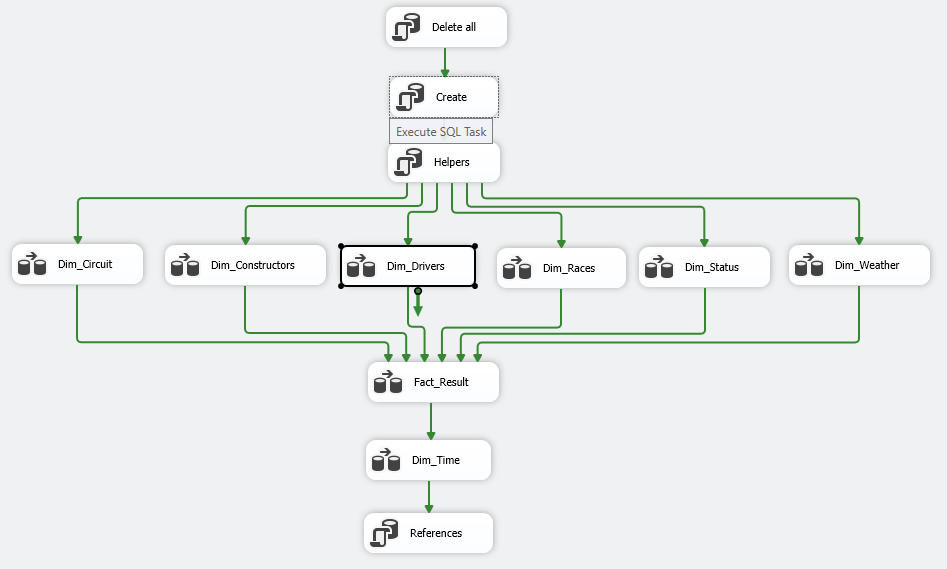
\includegraphics[width=0.8\textwidth]{etl.png}
  \caption{Cały ETL.}
\end{figure}

\begin{figure}[H]
  \centering
  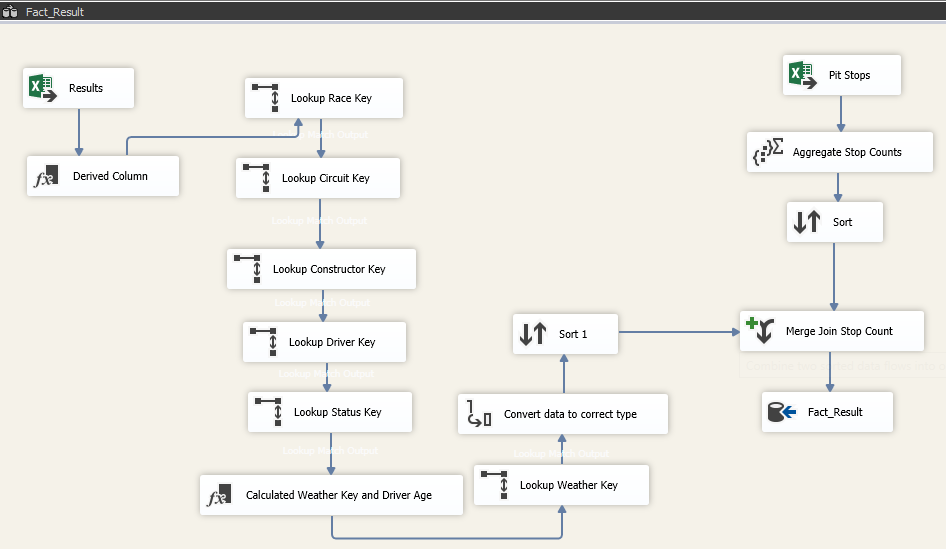
\includegraphics[width=0.8\textwidth]{result.png}
  \caption{ETL dla Fact\_Result.}
\end{figure}

\begin{figure}[H]
  \centering
  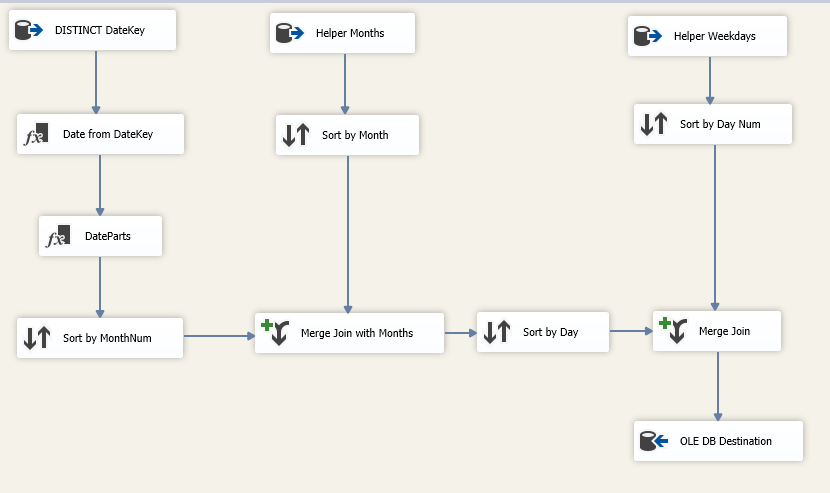
\includegraphics[width=0.8\textwidth]{time.png}
  \caption{ETL dla Dim\_Time.}
\end{figure}

\begin{figure}[H]
  \centering
  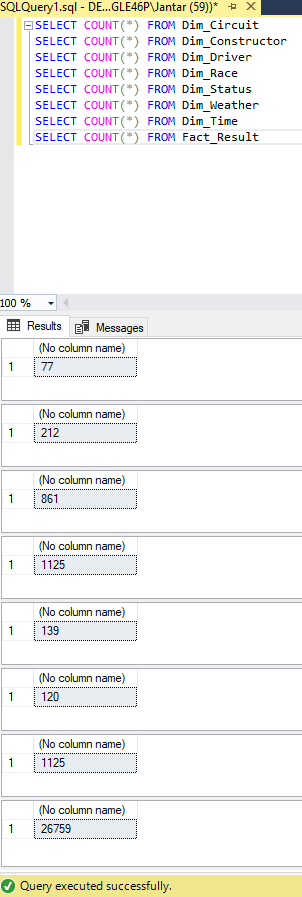
\includegraphics[width=0.8\textwidth]{final_counts.png}
  \caption{Liczby wierszy w wymiarach i fakcie - zgadzają się ze źródłem danych.}
\end{figure}

\subsection{Ekstrakcja danych (Extract)}
Dane źródłowe w formacie XLSX były wczytywane przy użyciu komponentu Excel Source w SSIS. Kluczowe aspekty konfiguracji tego etapu to:
\begin{itemize}
  \item Poprzednia konwersja plików .csv to .xlsx za pomocą skryptu Python, aby pominąć błędy w kodowaniu.
  \item Użycie skryptu Python do usunięcia "/N" w zbiorze danych.
  \item Poprawna identyfikacja separatorów kolumn, kwalifikatorów tekstu oraz obsługa wierszy nagłówkowych.
  \item Wstępne mapowanie typów danych na poziomie źródła, z uwzględnieniem późniejszych konwersji.
\end{itemize}

\subsection{Transformacja danych (Transform)}
Etap transformacji obejmował szereg operacji mających na celu oczyszczenie, integrację i przygotowanie danych do załadowania do tabel docelowych. Przykładowo:
\begin{enumerate}
  \item \textbf{Konwersja Typów Danych:} Komponent Data Conversion był wykorzystany do konwersji danych.
  \item \textbf{Obliczenia Pochodne:} Komponent Derived Column służył do tworzenia nowych kolumn na podstawie istniejących, np.:
        \begin{itemize}
          \item Obliczenie wieku kierowcy w momencie wyścigu (AgeAtRace).
          \item Obliczenie zmiany pozycji (PositionOrderChange).
        \end{itemize}
  \item \textbf{Agregacja Danych:}
        \begin{itemize}
          \item \textbf{Dane pogodowe (Dim\_Weather):} Minutowe dane pogodowe z pliku weather.xlsx były agregowane do poziomu pojedynczego wyścigu (po Year i RoundNumber) przy użyciu komponentu Aggregate. Obliczano wartości średnie, minimalne, maksymalne oraz sumy (np. dla opadów).
          \item \textbf{Dane o pit-stopach:} Informacje o liczbie i łącznym czasie pit-stopów dla każdego kierowcy w wyścigu były agregowane z pliku pit\_stops.xlsx i dołączane podczas ładowania tabeli faktów (np. poprzez wcześniejszą agregację do tabeli stagingowej i lookup).
        \end{itemize}
  \item \textbf{Kategoryzacja Danych Pogodowych:} Po agregacji, zagregowane wartości liczbowe dla danych pogodowych (np. temperatura, wilgotność, prędkość wiatru) były przekształcane na predefiniowane kategorie
        tekstowe (np. "Zimno", "Umiarkowanie", "Gorąco") przy użyciu wyrażeń warunkowych w komponencie Derived Column, zgodnie z założeniami projektu. Te kategorie zostały następnie załadowane do Dim\_Weather. Transformacja odbyła się w skrypcie C\#.
  \item \textbf{Fuzzy Lookup:} Do statusów dołączono ogólną kategorię statusu np. 'Mechanical Failure', 'Race Outcome' itd.
\end{enumerate}

\subsection{Ładowanie danych (Load)}
Przetransformowane dane były ładowane do docelowych tabel w hurtowni SQL Server przy użyciu komponentu OLE DB Destination.
\begin{itemize}
  \item Wykorzystano tryb szybkiego ładowania (Table or view - fast load).
  \item Zapewniono poprawne mapowanie kolumn z przepływu danych SSIS do kolumn tabel docelowych.
  \item Kolejność ładowania (najpierw wymiary, potem fakty) była zarządzana przez pakiet główny.
\end{itemize}

\subsection{Event handler}

W przypadku błędu, wszystkie dane są usuwane. Wcześniej podczas developmentu dodatkowo tabele były populowane, ponieważ wtedy występował błąd w metadanych SSIS.

\begin{figure}[H]
  \centering
  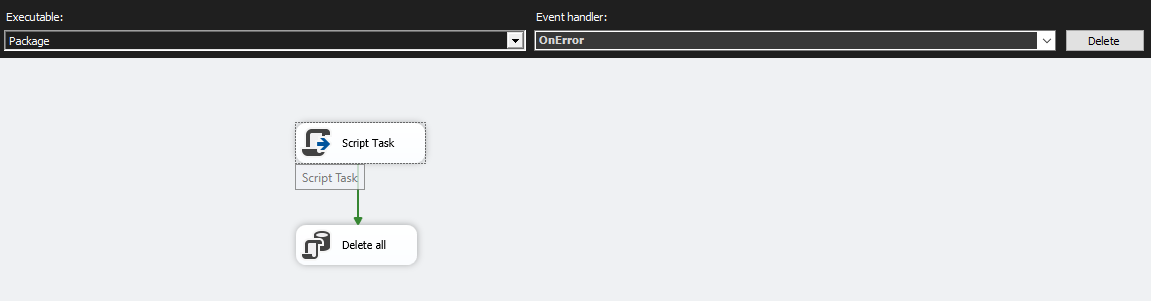
\includegraphics[width=0.8\textwidth]{error_handler.png}
  \caption{Error handler.}
\end{figure}

\subsection{Wyzwania i rozwiązania}
Podczas implementacji napotkano typowe wyzwania związane z procesami ETL:
\begin{itemize}
  \item \textbf{Niezgodność Stron Kodowych:} Początkowe problemy z konfliktem stron kodowych (np. 65001 z Flat File Source vs 1250 domyślne dla OLE DB Destination) zostały rozwiązane poprzez zmianę typu plików na Excel.
  \item \textbf{Synchronizacja Metadanych:} Zmiany w strukturze przepływu danych (np. po dodaniu Data Conversion) wymagały odświeżenia metadanych w komponencie OLE DB Destination i ponownego zmapowania kolumn.
  \item \textbf{Błędy Konwersji Danych w Źródle:} Błędy typu "Text was truncated or one or more characters had no match in the target code page" pojawiające się w Excel Source wskazywały na niepoprawną konfigurację strony kodowej dla pliku źródłowego. Trzeba było zmienić ręcznie w advanced editor dla źródła typy kolumn.
\end{itemize}

\section{Podsumowanie i wnioski z etapu ETL}
Proces ETL został pomyślnie zaimplementowany, umożliwiając zasilenie hurtowni danych Formuły 1 przetworzonymi i zintegrowanymi danymi. Kluczowe było właściwe zarządzanie typami danych i stronami kodowymi oraz logiczne rozplanowanie transformacji, w tym agregacji i kategoryzacji danych pogodowych. Zastosowanie SSIS pozwoliło na zbudowanie modularnego i zarządzalnego przepływu danych. Rozwiązane problemy z konwersją danych podkreślają znaczenie dokładnej analizy danych źródłowych i właściwej konfiguracji narzędzi ETL.

Kolejnym etapem będzie budowa kostki OLAP na bazie przygotowanej hurtowni danych oraz przeprowadzenie analiz wielowymiarowych.

\section{Projekt kostki OLAP}

\subsection{Struktura kostki}
Kostka OLAP, nazwana \texttt{FormulaCube}, została zbudowana w oparciu o tabelę faktów \texttt{Fact\_Result} oraz powiązane z nią tabele wymiarów, które zostały zdefiniowane i zasilone w poprzednich etapach projektu. Model kostki został zaprojektowany tak, aby umożliwić analitykom intuicyjne i efektywne korzystanie z danych. Wykorzystano schemat gwiazdy, gdzie centralna tabela faktów jest połączona z wymiarami.

\subsection{Wymiary kostki}
Kostka wykorzystuje następujące wymiary, które pozwalają na analizę danych z różnych perspektyw:
\begin{itemize}
  \item \textbf{Dim\_Driver:} Informacje o kierowcach.
  \item \textbf{Dim\_Constructor:} Informacje o zespołach konstruktorskich.
  \item \textbf{Dim\_Race:} Szczegóły dotyczące poszczególnych wyścigów.
  \item \textbf{Dim\_Circuit:} Informacje o torach wyścigowych.
  \item \textbf{Dim\_Time:} Hierarchia czasowa oparta na dacie wyścigu.
  \item \textbf{Dim\_Weather:} Skategoryzowane warunki pogodowe podczas wyścigu.
  \item \textbf{Dim\_Status:} Informacje o statusie ukończenia wyścigu przez kierowcę.
\end{itemize}

Występuje dodatkowo zdegenerowany wymiar z atrybutami dotyczącymi wieku kierowcy, pozycji startowej i końcowej.

\subsection{Hierarchie w wymiarach}
W celu ułatwienia analizy typu drill-down/roll-up, zdefiniowano następujące hierarchie w wymiarach:
\begin{itemize}
  \item \textbf{Dim\_Time (Hierarchia Czasowa):}
        \begin{itemize}
          \item Rok $\rightarrow$ Kwartał $\rightarrow$ Miesiąc $\rightarrow$ Dzień
        \end{itemize}
  \item \textbf{Dim\_Driver (Hierarchia Kierowcy):}
        \begin{itemize}
          \item Kontynent $\rightarrow$ Kraj
        \end{itemize}
  \item \textbf{Dim\_Constructor (Hierarchia Konstruktora):}
        \begin{itemize}
          \item Kontynent $\rightarrow$ Kraj
        \end{itemize}
  \item \textbf{Dim\_Circuit (Hierarchia Toru):}
        \begin{itemize}
          \item Kontynent $\rightarrow$ Kraj $\rightarrow$ Miasto $\rightarrow$ Nazwa Toru
        \end{itemize}
  \item \textbf{Dim\_Status (Hierarchia Statusu):}
        \begin{itemize}
          \item Kategoria Statusu $\rightarrow$ Opis Statusu
        \end{itemize}
\end{itemize}

\subsection{KPI}

W ramach kostki zdefiniowano \textbf{Constructor Reliability (Niezawodność Konstruktora):}

\begin{itemize}
  \item Wartość: 1 - DNF Percentage
  \item Cel: 80\%
  \item Status: Ocena, czy konstruktor osiąga zakładany poziom niezawodności
\end{itemize}

\begin{figure}[H]
  \centering
  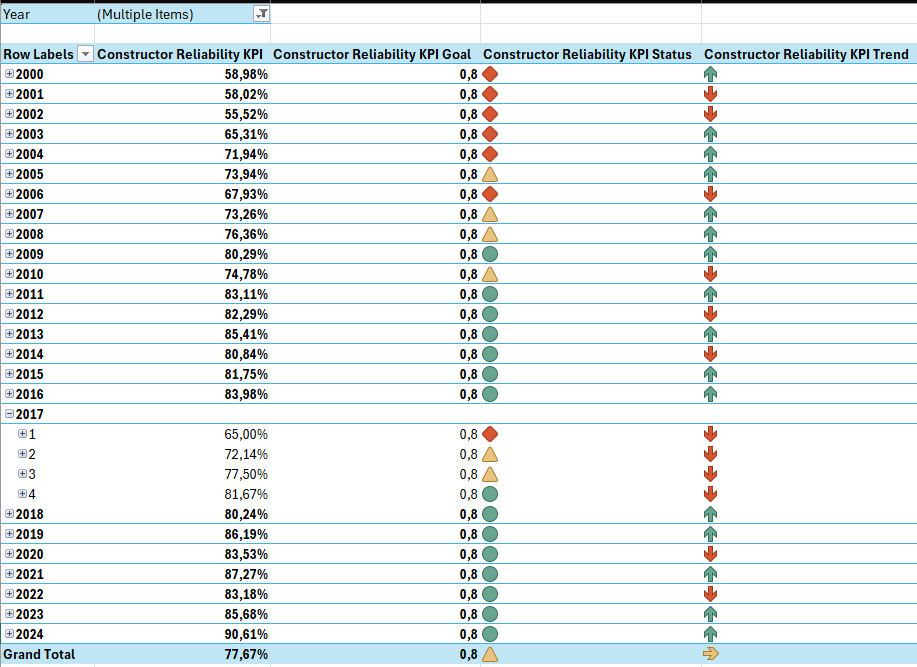
\includegraphics[width=0.9\textwidth]{kpi2.png}
  \caption{Widok KPI w latach 2000-2024.}
\end{figure}

Jak widać, kiedyś ta niezawodność nie była spełniona, natomiast przez ostatnie dwie dekady jest prawie zawsze spełniany.

\section{Implementacja kostki OLAP}
Kostka OLAP została zaimplementowana przy użyciu SQL Server Analysis Services (SSAS) 2019. Poniżej przedstawiono przykładowy widok struktury kostki oraz relacji wymiarów w SSAS.

\begin{figure}[H]
  \centering
  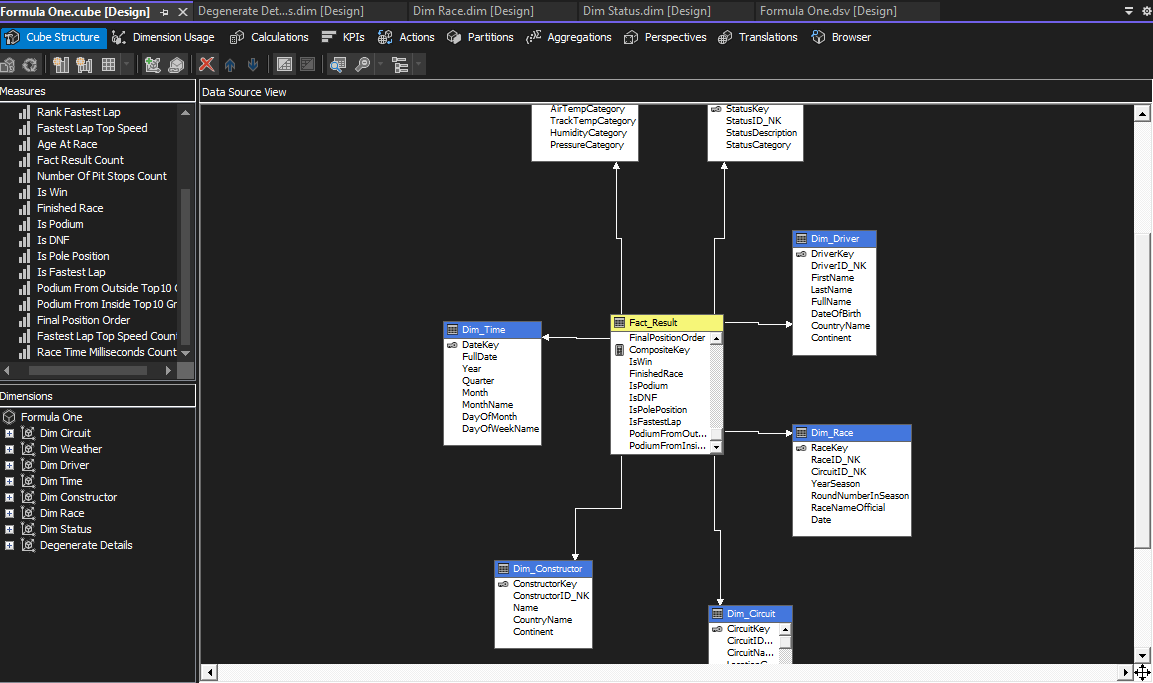
\includegraphics[width=0.9\textwidth]{cube_structure_placeholder.png}
  \caption{Widok struktury kostki.}
  \label{fig:cube_structure}
\end{figure}

\begin{figure}[H]
  \centering
  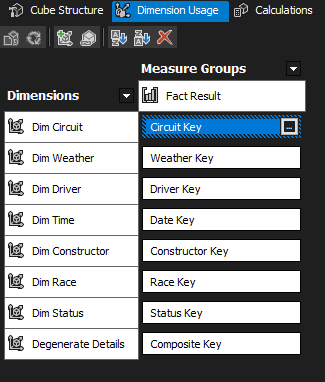
\includegraphics[width=0.9\textwidth]{dimension_usage_placeholder.png}
  \caption{Widok zakładki "Dimension Usage" w SQL Server Analysis Services.}
  \label{fig:dimension_usage}
\end{figure}

\section{Zestawienia wielowymiarowe i analizy}
Poniżej zaprezentowano zestawienia i wizualizacje wygenerowane na podstawie danych z kostki OLAP. Ilustrują one możliwości analityczne stworzonego rozwiązania.

\subsection{10 najczęstszych przyczyn awarii mechanicznych europejskich konstruktorów w latach 1950-1960}
\begin{figure}[H]
  \centering
  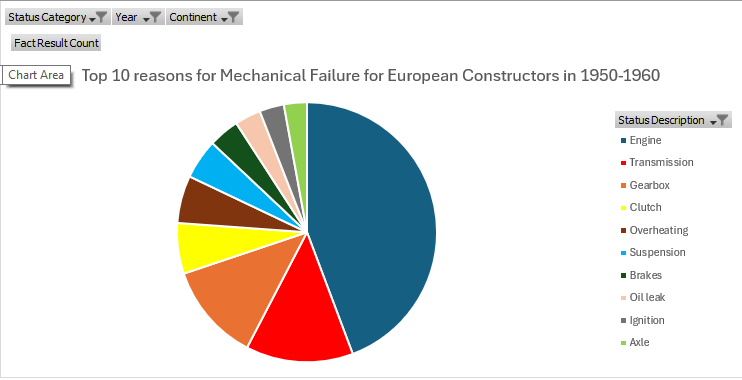
\includegraphics[width=0.8\textwidth]{Top 10 reasons for Mechanical Failure for European Constructors in 1950-1960.png}
\end{figure}
\textbf{Wnioski:} Problemy związane z silnikiem były zdecydowanie główną przyczyną awarii mechanicznych europejskich konstruktorów w latach 1950-1960. Problemy z układem przeniesienia napędu, skrzynią biegów oraz sprzęgłem były kolejnymi istotnymi, choć rzadszymi, przyczynami awarii.

\subsection{10 najczęstszych przyczyn awarii mechanicznych europejskich konstruktorów w latach 2010-2020}
\begin{figure}[H]
  \centering
  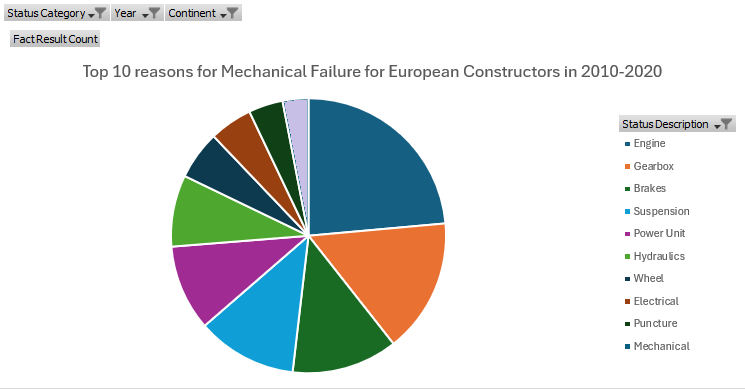
\includegraphics[width=0.8\textwidth]{Top 10 reasons for Mechanical Failure for European Constructors in 2010-2020.png}
\end{figure}
\textbf{Wnioski:} Problemy związane z silnikiem pozostały najczęstszą przyczyną awarii mechanicznych europejskich konstruktorów w latach 2010-2020. Awarie skrzyni biegów były drugą najczęstszą przyczyną. W porównaniu do okresu 1950-1960, "Power Unit" i "Hydraulics" pojawiły się jako istotne, odrębne kategorie awarii, odzwierciedlając postęp technologiczny i zmiany w konstrukcji samochodów. Problemy z hamulcami, zawieszeniem i układem elektrycznym również stanowiły znaczną część awarii mechanicznych.

\subsection{Średnia bezwzględna zmiana kolejności pozycji na torach w Austrii, Belgii, Francji i Niemczech}
\begin{figure}[H]
  \centering
  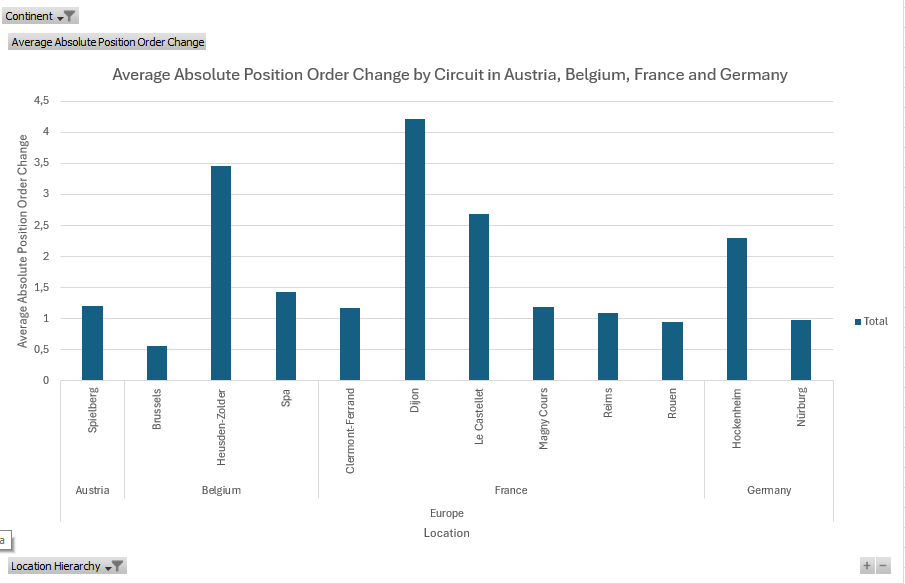
\includegraphics[width=0.8\textwidth]{Average Absolute Position Order Change by Circuit in Austria, Belgium, France and Germany.png}
\end{figure}
\textbf{Wnioski:} Wyścigi odbywające się na torze Dijon we Francji charakteryzowały się najwyższą średnią zmianą kolejności pozycji, co wskazuje na bardziej nieprzewidywalne wyścigi ze znacznymi przetasowaniami w stawce. Tor Heusden-Zolder w Belgii również odnotował znacząco wysoką średnią zmianę pozycji. Z kolei tory takie jak Spielberg, Clermont-Ferrand, Magny Cours, Reims, Rouen i Nürburgring wykazywały średnio porównywalnie mniejsze zmiany w kolejności wyścigu, a najmniej zmian występuje na torze w Brukseli.

\subsection{Średnia pozycja na mecie w zależności od pozycji startowej w Grand Prix Wielkiej Brytanii w latach 1990-2009}
\begin{figure}[H]
  \centering
  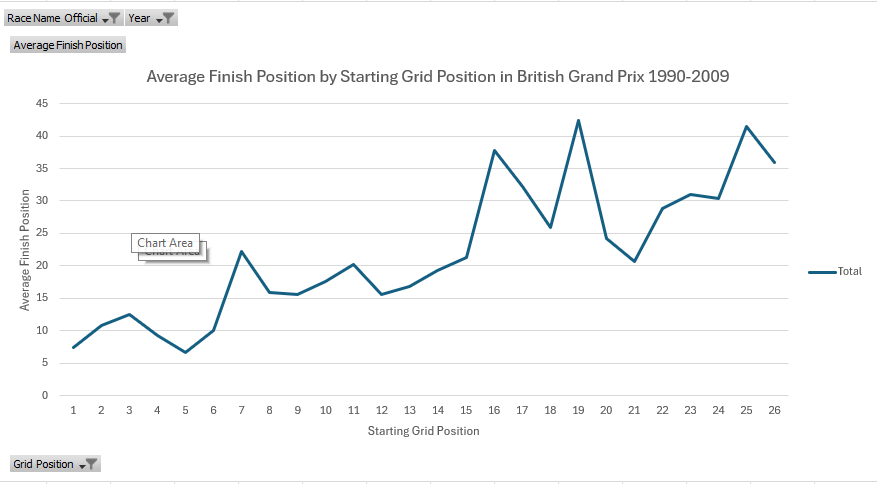
\includegraphics[width=0.8\textwidth]{Average Finish Position by Starting Grid Position in British Grand Prix 1990-2009.png}
\end{figure}
\textbf{Wnioski:} Ogólnie, wyższa pozycja startowa w Grand Prix Wielkiej Brytanii w latach 1990-2009 korelowała z wyższą średnią pozycją na mecie. Zależność ta nie była jednak idealnie liniowa, gdyż niektóre pozycje startowe (np. około 5.) osiągały lepsze wyniki niż pozycje bezpośrednio je poprzedzające, a niektóre dalsze pozycje startowe (np. około 19. i 24.) wykazywały szczególnie gorsze średnie wyniki na mecie.

\subsection{Procent DNF i średnia pozycja na mecie według grup wiekowych}
\begin{figure}[H]
  \centering
  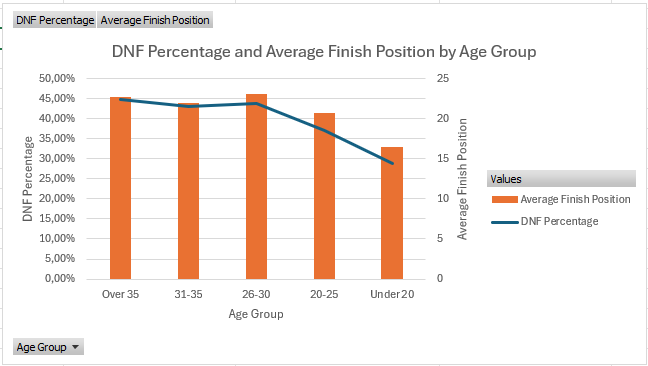
\includegraphics[width=0.8\textwidth]{DNF Percentage and Average Finish Position by Age Group.png}
\end{figure}
\textbf{Wnioski:} Młodsi kierowcy, szczególnie ci poniżej 20. roku życia, mieli tendencję do niższego odsetka DNF (nieukończeń wyścigu) i osiągania lepszych średnich pozycji na mecie. Kierowcy od 26. roku życia do powyżej 35. roku życia doświadczali najwyższych wskaźników DNF i najmniej korzystnych średnich pozycji na mecie. Ogólnie jest tendencja, że wraz ze wzrostem wieku kierowcy, wskaźniki DNF rosną, a średnie pozycje na mecie pogarszają się - jest ona najbardziej prawdziwa dla 3. grup wiekowych: under 20, 20-25 i 26-30.

\subsection{Procent zwycięstw i średnia prędkość najszybszego okrążenia według grup wiekowych}
\begin{figure}[H]
  \centering
  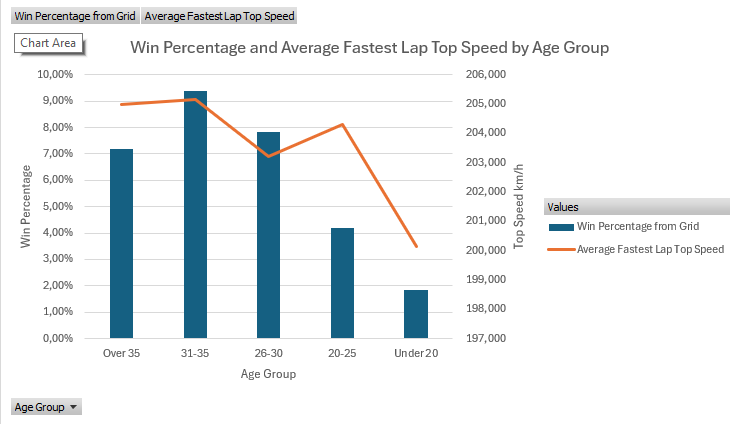
\includegraphics[width=0.8\textwidth]{Win Percentage and Average Fastest Lap Top Speed by Age Group.png}
\end{figure}
\textbf{Wnioski:} Kierowcy w grupie wiekowej 31-35 lat osiągali najwyższy procent zwycięstw ze swoich pozycji startowych, a także notowali najwyższe średnie prędkości najszybszych okrążeń. Procenty zwycięstw były znacznie niższe dla młodszych grup wiekowych (poniżej 20 lat i 20-25 lat). Chociaż kierowcy powyżej 35. roku życia mieli drugą najwyższą średnią prędkość, ich procent zwycięstw był niższy niż w grupie wiekowej 26-30 lat. Jest to ciekawa różnica w porównaniu do poprzedniej analizy, gdzie najmłodsi kierowcy osiągali lepsze wyniki. Należy pamiętać, że było bardzo niewielu kierowców under 20, przez co mogło nastąpić przeszacowanie umiejętności.

\subsection{Procent ukończeń wyścigu według kategorii pogodowych}
\begin{figure}[H]
  \centering
  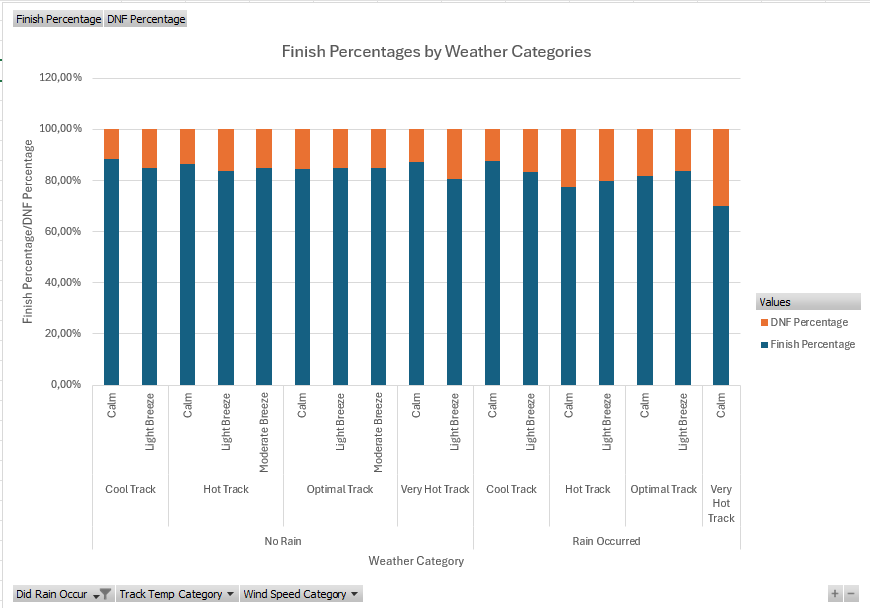
\includegraphics[width=0.8\textwidth]{Finish Percentages by Weather Categories.png}
\end{figure}
\textbf{Wnioski:} We wszystkich wymienionych kategoriach pogodowych (kombinacje temperatury toru, deszczu i warunków wietrznych) zdecydowana większość startujących pomyślnie ukończyła wyścigi. Występują jednak różnice - największy procent DNF wystąpił dla najgorszych warunków pogodowych, czyli gorąca powierzchnia i deszcz. Generalnie sam deszcz lekko wpływa na zwiększenie procentu DNF. Nie wygląda na to, że gdy nie pada, temperatura track ma wielki wpływ na DNF - chociaż najmniej DNF odbyło się przy najlepszych możliwych warunkach pogodowych - brak wiatru, zimna nawierzchnia i brak deszczu.

\subsection{Top 5 konstruktorów według średniej liczby punktów}
\begin{figure}[H]
  \centering
  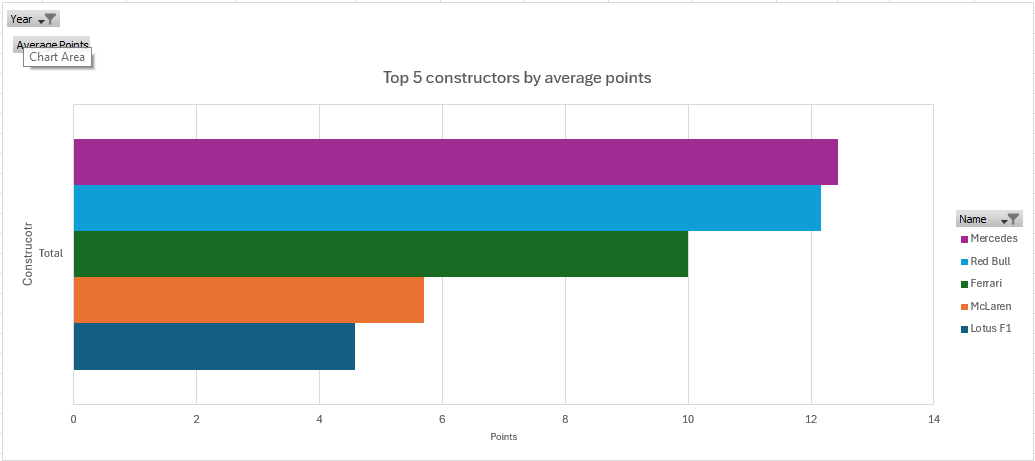
\includegraphics[width=0.8\textwidth]{Top 5 constructors by average points.png}
\end{figure}
\textbf{Wnioski:} Mercedes był najlepszym konstruktorem pod względem średniej liczby punktów, wyprzedzając Red Bulla, a następnie Ferrari. McLaren i Lotus F1 zajęły odpowiednio czwarte i piąte miejsce, ale ze znaczącą niższą średnią liczbą punktów w porównaniu do pierwszej trójki.

\subsection{Procent zwycięstw na przestrzeni lat 2018-2024 dla 9 najlepszych kierowców w Europie}
\begin{figure}[H]
  \centering
  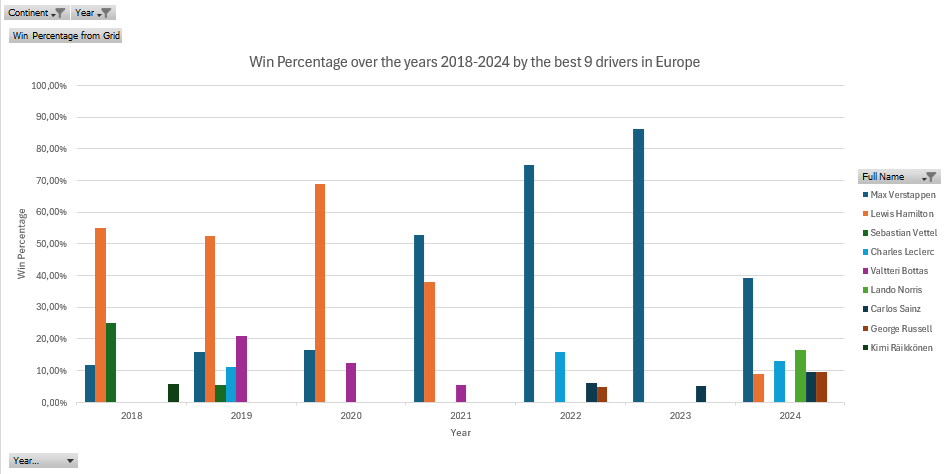
\includegraphics[width=0.8\textwidth]{Win Percentage over the years 2018-2024 by the best 9 drivers in Europe.png}
\end{figure}
\textbf{Wnioski:} Procent zwycięstw Maxa Verstappena wykazywał znaczący trend wzrostowy od 2018 do 2023 roku, kulminując dominującym występem w 2023 roku. Lewis Hamilton wykazywał wysokie odsetki zwycięstw we wcześniejszych latach (2018-2020), ale w kolejnych latach odnotował spadek. Inni kierowcy mieli sporadyczne lub niższe odsetki zwycięstw, przy czym Verstappen wyraźnie wyrósł na najbardziej utytułowanego zawodnika tej grupy w późniejszej części okresu. Dane za 2024 rok pokazują bardziej wyrównane wyniki dla kierowców, poza Maxem, który co prawda był słabszy niż w 2023, ale dalej najlepszy.

\subsection{Średnia liczba pit stopów w zależności od występowania deszczu w latach 2018-2023}
\begin{figure}[H]
  \centering
  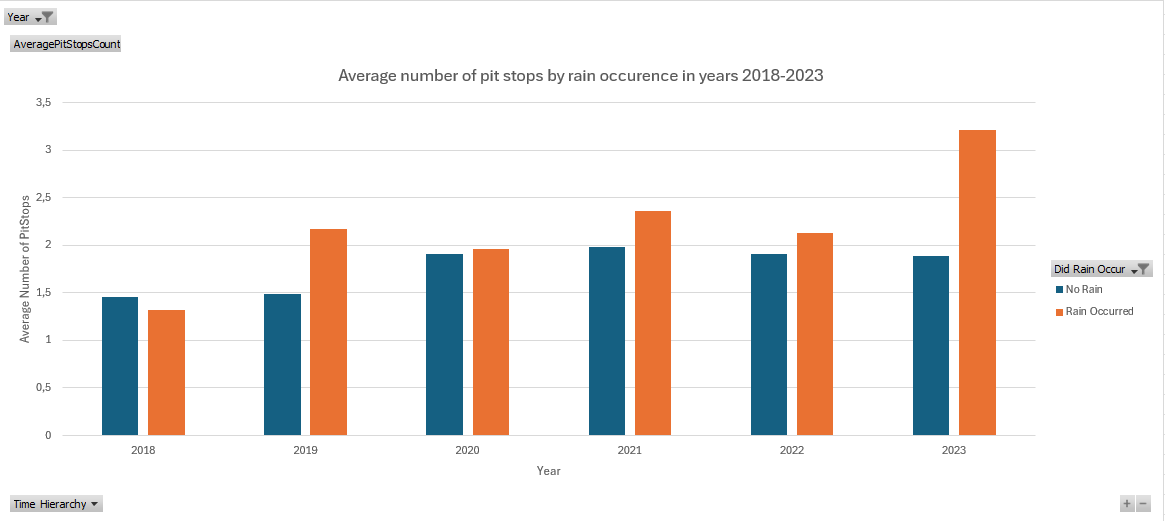
\includegraphics[width=0.8\textwidth]{Average number of pit stops by rain occurence in years 2018-2023.png}
\end{figure}
\textbf{Wnioski:} Występowanie deszczu konsekwentnie prowadziło do wyższej średniej liczby pit stopów w wyścigach w latach 2018-2023. W każdym obserwowanym roku wyścigi, na które wpłynął deszcz, charakteryzowały się średnio większą liczbą pit stopów w porównaniu do wyścigów bez niego. Co więcej, odnotowano niewielki trend wzrostowy średniej liczby pit stopów w warunkach deszczowych od 2018 do 2023 roku, osiągając szczyt w 2023 roku. Właśnie w 2023 liczba pit stopów była zdecydowanie najwyższa, gdy padał deszcz.

\subsection{Średni czas wyścigu na torze Autodromo Nazionale di Monza według roku}
\begin{figure}[H]
  \centering
  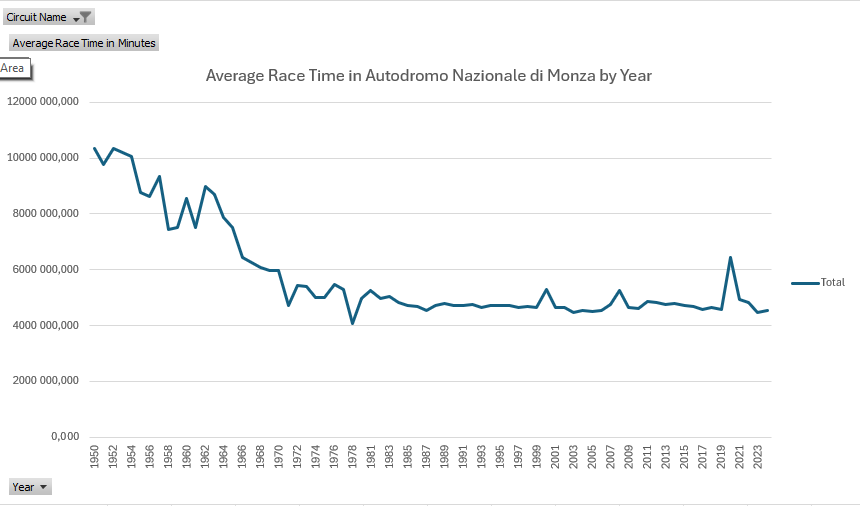
\includegraphics[width=0.8\textwidth]{Average Race Time in Autodromo Nazionale di Monza by Year.png}
\end{figure}
\textbf{Wnioski:} Nastąpił radykalny spadek średnich czasów wyścigów na torze Autodromo Nazionale di Monza od 1950 roku do późnych lat 70. Po tym okresie gwałtownej poprawy prędkości lub wydajności wyścigów, średni czas wyścigu w dużej mierze ustabilizował się, wykazując jedynie niewielkie wahania do 2023 roku, z zauważalnym wzrostem w 2020 roku. Występowały też niewielkie wzrosty w 2008 i w 2000 roku. Z danych wcześniej analizowanych wynikałoby, że w 2023 roku deszcze wpłynęły mocno na pit stopy.

\subsection{Podium z pierwszej dziesiątki lub spoza pierwszej dziesiątki pól startowych według kategorii deszczu i wiatru}
\begin{figure}[H]
  \centering
  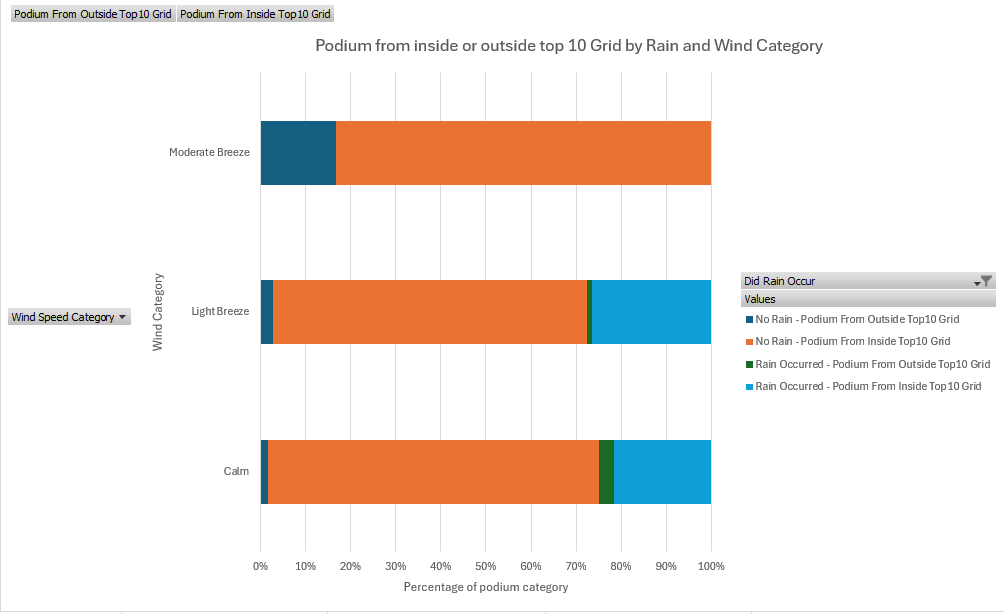
\includegraphics[width=0.8\textwidth]{Podium from inside or outside top 10 Grid by Rain and Wind Category.png}
\end{figure}
\textbf{Wnioski:} Start z pierwszej dziesiątki pól startowych znacząco zwiększał prawdopodobieństwo ukończenia wyścigu na podium w większości warunków, szczególnie przy pogodzie bez silniejszego wiatru. Jednakże wystąpienie deszczu, szczególnie bez wiatru, zauważalnie zwiększało odsetek zawodników kończących na podium, którzy startowali spoza pierwszej dziesiątki pól startowych. Sugeruje to, że warunki deszczowe, zwłaszcza przy braku wiatru, tworzą bardziej nieprzewidywalne wyścigi, w których pozycja startowa jest mniej decydującym czynnikiem osiągnięcia podium. Największy procent podium spoza pierwszej dziesiątki występował jednak wtedy, kiedy wiatr był dość silny.

\newpage
\section{Dokumentacja kostki}

\subsection{Opis wymiarów i atrybutów}

\subsubsection{Dim\_Driver (Kierowca)}
\begin{itemize}
  \item \textbf{Atrybuty:}
        \begin{itemize}
          \item DriverKey (PK, Klucz Zastępczy)
          \item DriverID\_NK (Klucz Naturalny ze źródła)
          \item FirstName (Imię)
          \item LastName (Nazwisko)
          \item FullName (Pełne Imię i Nazwisko) - używane w hierarchii
          \item DateOfBirth (Data Urodzenia)
          \item CountryName (Kraj pochodzenia) - używane w hierarchii
          \item Continent (Kontynent pochodzenia) - używane w hierarchii
        \end{itemize}
  \item \textbf{Hierarchie:} Kontynent $\rightarrow$ Kraj
\end{itemize}

\subsubsection{Dim\_Constructor (Konstruktor)}
\begin{itemize}
  \item \textbf{Atrybuty:}
        \begin{itemize}
          \item ConstructorKey (PK, Klucz Zastępczy)
          \item ConstructorID\_NK (Klucz Naturalny ze źródła)
          \item Name (Nazwa Konstruktora) - używane w hierarchii
          \item CountryName (Kraj pochodzenia) - używane w hierarchii
          \item Continent (Kontynent pochodzenia) - używane w hierarchii
        \end{itemize}
  \item \textbf{Hierarchie:} Kontynent $\rightarrow$ Kraj
\end{itemize}

\subsubsection{Dim\_Race (Wyścig)}
\begin{itemize}
  \item \textbf{Atrybuty:}
        \begin{itemize}
          \item RaceKey (PK, Klucz Zastępczy)
          \item RaceID\_NK (Klucz Naturalny ze źródła)
          \item CircuitID\_NK (Klucz Naturalny toru dla tego wyścigu)
          \item YearSeason (Rok Sezonu)
          \item RoundNumberInSeason (Numer Rundy w Sezonie)
          \item RaceNameOfficial (Oficjalna Nazwa Wyścigu)
          \item Date (Data Wyścigu) - używana do połączenia z Dim\_Time
        \end{itemize}
  \item \textbf{Hierarchie:} Brak zdefiniowanych (możliwe: Rok Sezonu $\rightarrow$ Nazwa Wyścigu)
\end{itemize}

\subsubsection{Dim\_Circuit (Tor)}
\begin{itemize}
  \item \textbf{Atrybuty:}
        \begin{itemize}
          \item CircuitKey (PK, Klucz Zastępczy)
          \item CircuitID\_NK (Klucz Naturalny ze źródła)
          \item CircuitName (Nazwa Toru) - używane w hierarchii
          \item LocationCity (Miasto) - używane w hierarchii
          \item CountryName (Kraj) - używane w hierarchii
          \item Continent (Kontynent) - używane w hierarchii
        \end{itemize}
  \item \textbf{Hierarchie:} Kontynent $\rightarrow$ Kraj $\rightarrow$ Miasto $\rightarrow$ Nazwa Toru
\end{itemize}

\subsubsection{Dim\_Time (Czas)}
\begin{itemize}
  \item \textbf{Atrybuty:}
        \begin{itemize}
          \item DateKey (PK, format YYYYMMDD)
          \item FullDate (Pełna data, typ Date)
          \item Year (Rok) - używane w hierarchii
          \item Quarter (Kwartał) - używane w hierarchii
          \item Month (Miesiąc numer) - używane w hierarchii
          \item MonthName (Nazwa Miesiąca)
          \item DayOfMonth (Dzień Miesiąca) - używane w hierarchii jako najniższy poziom
          \item DayOfWeekName (Nazwa Dnia Tygodnia)
        \end{itemize}
  \item \textbf{Hierarchie:} Rok $\rightarrow$ Kwartał $\rightarrow$ Miesiąc $\rightarrow$ Dzień (FullDate)
\end{itemize}

\subsubsection{Dim\_Weather (Pogoda)}
\begin{itemize}
  \item \textbf{Atrybuty:}
        \begin{itemize}
          \item WeatherKey (PK, np. Rok * 100 + Runda)
          \item DidRainOccur (Czy wystąpił deszcz: "Rain Occurred"/"No Rain")
          \item WindSpeedCategory (Kategoria Prędkości Wiatru: np. "Light Breeze", "Calm")
          \item AirTempCategory (Kategoria Temperatury Powietrza: np. "Cold", "Warm")
          \item TrackTempCategory (Kategoria Temperatury Toru: np. "Optimal Track", "Very Hot Track")
          \item HumidityCategory (Kategoria Wilgotności: np. "Dry", "Humid")
          \item PressureCategory (Kategoria Ciśnienia: np. "Very Low", "Normal")
        \end{itemize}
  \item \textbf{Hierarchie:} Brak zdefiniowanych (każdy atrybut jest osobną "mini-hierarchią")
\end{itemize}

\subsubsection{Dim\_Status (Status ukończenia)}
\begin{itemize}
  \item \textbf{Atrybuty:}
        \begin{itemize}
          \item StatusKey (PK, Klucz Zastępczy)
          \item StatusID\_NK (Klucz Naturalny ze źródła)
          \item StatusDescription (Opis Statusu) - używane w hierarchii
          \item StatusCategory (Ogólna Kategoria Statusu, np. "Race Outcome", "Mechanical Failure") - używane w hierarchii
        \end{itemize}
  \item \textbf{Hierarchie:} Kategoria Statusu $\rightarrow$ Opis Statusu
\end{itemize}

\subsubsection{Dim\_DegenerateDetails (Wymiar zdegenerowany)}
\begin{itemize}
  \item \textbf{Atrybuty:}
        \begin{itemize}
          \item CompositeKey (PK, Klucz Zastępczy)
          \item AgeAtRace (Wiek Kierowcy w momencie wyścigu)
          \item AgeGroup (Grupa wiekowa, np. "Under 20", "20-25")
          \item GridPosition (Pozycja Startowa)
          \item FinalPositionOrder (Końcowa Pozycja w Wyścigu)
        \end{itemize}
\end{itemize}

\subsection{Miary}

\subsubsection*{Miary pochodzące bezpośrednio z tabeli faktów}

\begin{enumerate}[label=\arabic*., wide, labelindent=0pt]
  \item \textbf{Points Scored:} Liczba punktów zdobytych przez kierowcę w wyścigu.
  \item \textbf{Laps Completed:} Liczba ukończonych okrążeń.
  \item \textbf{Number of Pit Stops:} Sumaryczna liczba wykonanych pit stopów.
  \item \textbf{Race Time Milliseconds:} Sumaryczny czas wyścigu w milisekundach (dla tych, co ukończyli i mają zarejestrowany czas).
  \item \textbf{Grid Position:} Pozycja startowa kierowcy.
  \item \textbf{Final Position Order:} Końcowa pozycja kierowcy w wyścigu.
  \item \textbf{Position Order Change:} Zmiana pozycji (pozycja startowa - pozycja końcowa).
  \item \textbf{Rank Fastest Lap:} Ranking najszybszego okrążenia kierowcy w danym wyścigu.
  \item \textbf{Fastest Lap Top Speed:} Prędkość maksymalna osiągnięta podczas najszybszego okrążenia.
  \item \textbf{Is Win:} Suma flag (0/1) wskazujących na zwycięstwo.
  \item \textbf{Finished Race:} Suma flag (0/1) wskazujących na ukończenie wyścigu.
  \item \textbf{Is Podium:} Suma flag (0/1) wskazujących na miejsce na podium.
  \item \textbf{Is DNF:} Suma flag (0/1) wskazujących na nieukończenie wyścigu (Did Not Finish).
  \item \textbf{Is Pole Position:} Suma flag (0/1) wskazujących na zdobycie pole position.
  \item \textbf{Is Fastest Lap:} Suma flag (0/1) wskazujących na zdobycie najszybszego okrążenia.
  \item \textbf{Podium From Outside Top 10 Grid:} Suma flag (0/1) wskazujących na podium ze startu spoza TOP 10.
  \item \textbf{Podium From Inside Top 10 Grid:} Suma flag (0/1) wskazujących na podium ze startu z TOP 10.
\end{enumerate}

\subsubsection*{Miary kalkulowane}

\begin{enumerate}[label=\arabic*., wide, labelindent=0pt]
  \item \textbf{Race Time Formatted:} Sformatowany czas wyścigu dla czytelności.
  \item \textbf{Absolute Position Order Change:} Bezwzględna wartość zmiany pozycji (start vs meta).
  \item \textbf{Average PitStops Count:} Średnia liczba pit stopów na występ kierowcy, który miał odnotowane pit stopy.
  \item \textbf{Average Absolute Position Order Change:} Średnia bezwzględna zmiana pozycji na start.
  \item \textbf{Average Points:} Średnia liczba zdobytych punktów na start.
  \item \textbf{Number of Wins:} Całkowita liczba zwycięstw. Jawne zdefiniowanie sumy miary bazowej \texttt{IsWin}.
  \item \textbf{Average Finish Position:} Średnia pozycja na mecie dla kierowców, którzy ukończyli wyścig.
  \item \textbf{Win Percentage from Grid:} Procent wygranych spośród wszystkich rozpoczętych wyścigów.
  \item \textbf{Finish Percentage:} Procent ukończonych wyścigów spośród wszystkich startów.
  \item \textbf{DNF Percentage:} Procent nieukończonych wyścigów (DNF) spośród wszystkich startów.
  \item \textbf{Average Fastest Lap Top Speed:} Średnia maksymalna prędkość na najszybszym okrążeniu (dla tych, którzy je odnotowali).
  \item \textbf{Average Race Time in Minutes:} Średni czas wyścigu w minutach.
  \item \textbf{Age At Race:} Średni wiek kierowcy w momencie wyścigu.
\end{enumerate}

\section{Wnioski z analizy danych}

Przeprowadzone analizy na kostce OLAP pozwoliły na wyciągnięcie kilku interesujących wniosków oraz zaobserwowanie zależności:

\begin{itemize}
  \item Ewolucja awarii mechanicznych: Silnik konsekwentnie pozostaje główną przyczyną awarii na przestrzeni dekad (1950-60 vs 2010-20). Jednak pojawienie się kategorii "Power Unit" i "Hydraulics" w nowszym okresie, obok nadal istotnych problemów ze skrzynią biegów, hamulcami czy zawieszeniem, doskonale ilustruje wzrost złożoności technologicznej współczesnych bolidów i integrację systemów hybrydowych oraz zaawansowanych systemów pomocniczych.
  \item Nieprzewidywalność wyścigów a charakterystyka toru i pogoda: Tory takie jak Dijon czy Zolder, ze względu na swoją charakterystykę, generują bardziej dynamiczne i nieprzewidywalne wyścigi (więcej zmian pozycji). Jednocześnie, warunki deszczowe, albo silniejszy wiatr, znacząco zwiększają szansę na podium dla kierowców startujących spoza pierwszej dziesiątki.
  \item Związek wieku kierowcy z wynikami: Młodsi kierowcy (<20 lat) mają mniej DNF i lepsze średnie pozycje, co może być efektem tego, że do F1 w tak młodym wieku trafiają wybitne talenty, często od razu do czołowych zespołów (choć mała liczebność grupy może wpływać na te dane). Jednak szczytową formę pod względem procentu zwycięstw i prędkości najszybszych okrążeń osiągają kierowcy w wieku 31-35 lat, co wskazuje na idealne połączenie doświadczenia, dojrzałości taktycznej i wciąż wysokich zdolności fizycznych. Starsze grupy wiekowe (26+) generalnie częściej nie kończą wyścigów i mają gorsze średnie pozycje.
  \item Dominacja konstruktorów i kierowców: Analiza konstruktorów (Mercedes, Red Bull, Ferrari na czele) i procentu zwycięstw kierowców (dominacja Hamiltona, a potem Verstappena) wyraźnie pokazuje okresy dominacji poszczególnych zespołów i zawodników. Dane z 2024 sugerują potencjalne zaciśnięcie się czołówki, choć Verstappen nadal utrzymuje silną pozycję.
  \item Wpływ deszczu na strategię: Deszcz nie tylko zwiększa ryzyko DNF i nieprzewidywalność (podium spoza TOP10), ale także konsekwentnie prowadzi do większej liczby pit stopów. Ciekawy jest trend wzrostowy liczby pit stopów w deszczu w latach 2018-2023, co może świadczyć o ewolucji strategii lub częstszych neutralizacjach w takich warunkach.
  \item Postęp technologiczny a czasy wyścigów: Drastyczny spadek średnich czasów wyścigów na torze Monza do końca lat 70. XX wieku obrazuje skokowy postęp technologiczny w F1. Późniejsza stabilizacja czasów (z niewielkimi fluktuacjami, np. wzrost w 2020) może świadczyć o osiągnięciu pewnego plateau wydajnościowego w ramach obowiązujących regulacji, większym nacisku na bezpieczeństwo lub o tym, że sam tor nie przechodził modyfikacji znacząco skracających czas okrążenia.
\end{itemize}

Stworzona kostka OLAP jest dobrym narzędziem do dalszej, pogłębionej eksploracji danych, umożliwiając zadawanie złożonych pytań i odkrywanie ukrytych wzorców.

\end{document}